\documentclass[journal=cmatex,manuscript=perspective]{achemso}

\usepackage[version=3]{mhchem} % Formula subscripts using \ce{}
\usepackage[T1]{fontenc}       % Use modern font encodings
\usepackage{siunitx}           % Numbers with units, eg. 1.6 mm
\usepackage{textcomp}          % Special symbols for text mode

%% Needed only for highlighting during draft process
%% Remove for final copy
\usepackage{xcolor}
\usepackage{soul}

%% Use one of these two lines for links
\usepackage{hyperref}            % Special formatting for hyperlinks
% \usepackage[hidelinks]{hyperref} % No formatting for hyperlinks

%% Meta-data author info
\author{Mark Wolf}
\author{Brian M. May}
\author{Jordi Cabana}
\email{jcabana@uic.edu}
\affiliation[University of Illinois at Chicago]
{Department of Chemistry, University of Illinois at Chicago, Chicago IL}

\title{Visualization of Electrochemical Reactions in Battery Materials
  with X-ray Microscopy and Mapping}

%% Macro to indicated permission to reproduce figures from IUCr
\newcommand{\iucr}{Reproduced with permission of the
  \href{http://journals.iucr.org/}{International Union of
    Crystallography}.}

\begin{document}

\begin{tocentry}
  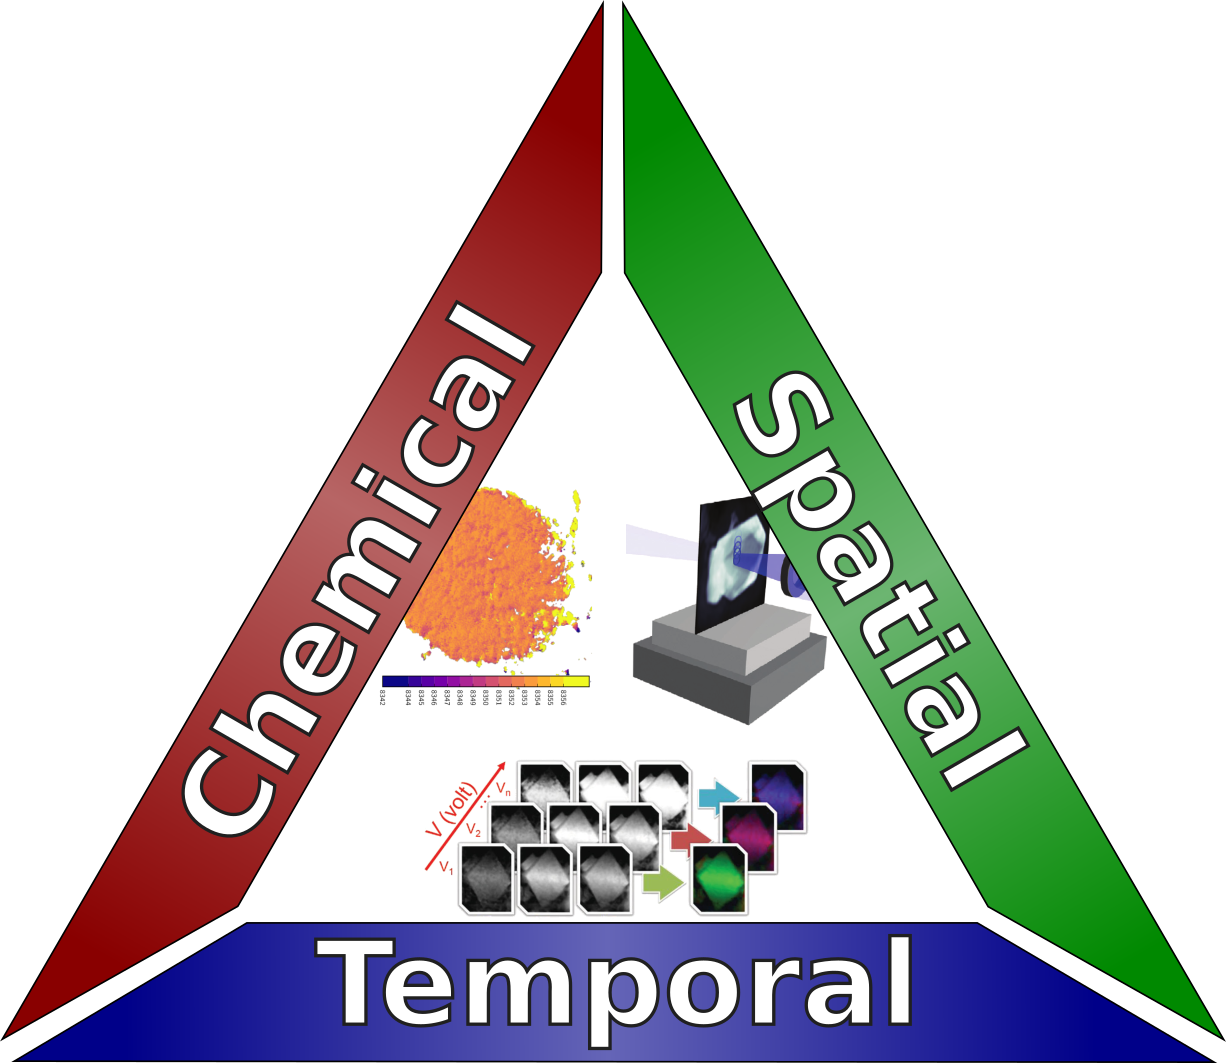
\includegraphics[height=1.375in]{resolution-triangle.png}
\end{tocentry}

\begin{abstract}
  Unlocking the full performance capabilities of battery materials
  will require a thorough understanding of the underlying
  electrochemical mechanisms at a variety of length scales. A broad
  arsenal of X-ray microscopy and mapping techniques is now available
  to probe these processes down to the nano-scale. The tunable nature
  of X-ray sources allows for the extraction of chemical states
  through spectromicroscopy. The addition of phase contrast imaging
  can retrieve the complex-valued refraction of the material, giving
  an even more nuanced chemical picture. Tomography and coherent Bragg
  diffraction imaging provide a reconstructed three-dimensional volume
  of the specimen, as well as internal strain information from the
  latter. Many recent insights into battery materials have been
  achieved through the creative use of these, and similar,
  methods. Experiments performed while the battery is being actively
  cycled reveal behavior that differs significantly from what is
  observed at equilibrium and meta-stable conditions. Planned
  improvements to X-ray source brightness and coherence will extend
  these techniques by alleviating the current trade-off in time,
  chemical and spatial resolution.
\end{abstract}

\section{Introduction}

Beyond the visible consumer electronics applications, energy storage
plays a critical role in areas such as manufacturing, transportation
and electricity generation. By some estimates, US industries lose \$80
billion each year due to power interruptions, while annual electric
vehicle sales are seeing large and consistent
increases\cite{whittingham2012}. Additionally, if renewables are to
become the main source of energy production, we will need storage
solutions to deal with their intermittent nature. Even with coal and
natural gas, fluctuations in demand require that more expensive
``peaker plants'' be brought online, which could be alleviated if
energy from base-load plants can be stored when demand is low. The
cheapest energy storage methods, pumped-hydro and compressed-air, are
severely limited by the availability of suitable locations. Currently,
batteries hold much promise as portable energy storage
systems. Batteries contain two electrodes, sites where oxidation and
reduction reactions (redox) take place\cite{armand2008}. The
fundamental redox chemistry within batteries is non-trivial and
governs the practical aspects that are felt by the consumer, such as
capacity, cycle life, and power, among others. Therefore, advances in
battery technology that yield cheaper, more reliable and better
performing systems will result in large economic, environmental and
geopolitical benefits. A key requirement for achieving this goal is a
better understanding of the chemistry underlying these materials, in
order to operate as close as possible to their theoretical limits.

Measuring chemical properties with spatial resolution provides a view
of the underlying mechanisms that is not available by looking at bulk
properties. Electrodes generally adopt a hierarchical structure
wherein single crystallites of a redox-active material combine to form
agglomerate particles, which are then combined with conductive
additives and flexible polymeric binders into a thick (ideally, above
\SI{100}{\micro\metre}), porous electrode architecture (figure
\ref{figure:multiscale-1}) where different distributions of components
and particle sizes are likely to exist throughout the electrode,
demonstrated in figure \ref{figure:multiscale-2}. In addition, the
thickness of the electrode introduces asymmetries in the transport of
ions (from the electrolyte) and electrons (from the current collector,
figure \ref{figure:multiscale-2}), which are both required in order
for the redox reaction to proceed. As a result, a hierarchy of
inhomogeneities develops during the phase transformation, both within
the electrode\cite{newman1995,srinivasan2014} and within individual
particles. These inhomogeneities are kinetic in origin, beyond the
changes that would be inherent to the phase transformation within a
particle, and, thus, prone to vary with the currents to which the
battery is subjected. Probing all of these length-scales provides
clues for helping meet the high demands placed on current technology.

\begin{figure}
  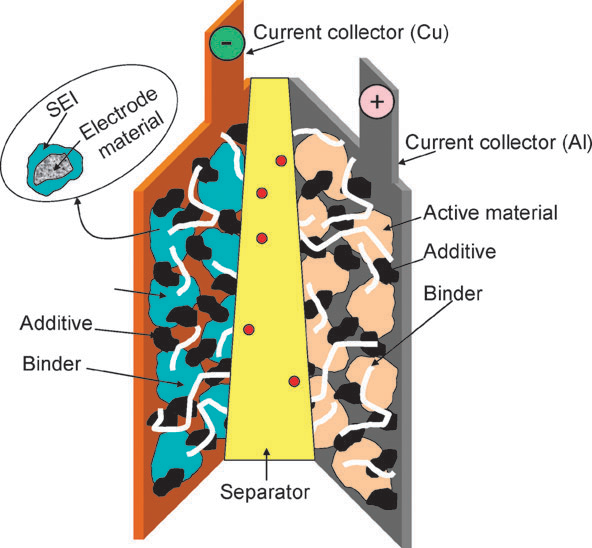
\includegraphics[width=\textwidth]{multiscale-1.png}
  \caption{Schematic of a typical battery. The electrodes are made of
    multiple individual particles that participate in the
    electrochemical reaction (denoted as ``active
    material''). Reproduced from Ref.\cite{palacin2009} with
    permission from the Royal Society of Chemistry.}
  \label{figure:multiscale-1}
\end{figure}

\begin{figure}
  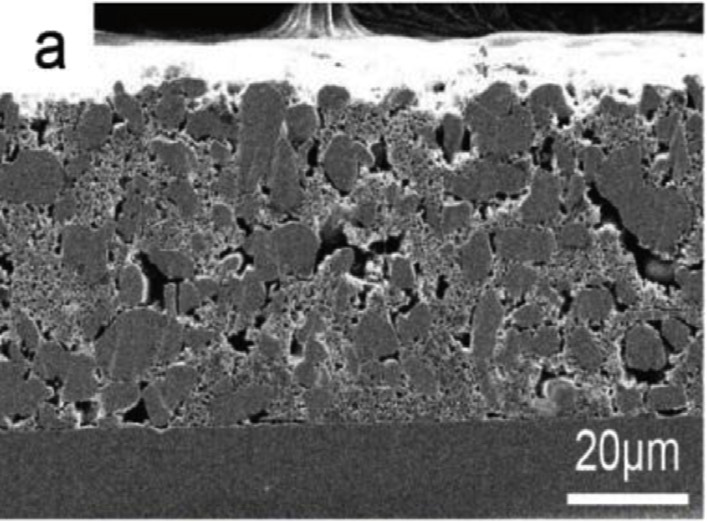
\includegraphics[width=\textwidth]{multiscale-2.png}
  \caption{Scanning electron microscope image of the cross-section of
    a typical battery electrode. Multiple individual particles can be
    seen that participate in the electrochemical reaction. Reprinted
    from Journal of \textit{Power Sources}, \textit{252}, J. Choi et
    al., Improved high-temperature performance of lithium-ion
    batteries through use of a thermally stable co-polyimide-based
    cathode binder, 138-143, \textbf{2014}, with permission from
    Elsevier.}
  \label{figure:multiscale-2}
\end{figure}

X-rays are able to probe various length scales using a variety of
contrast mechanisms. Compared to electron microscopy, another common
tool for achieving spatially resolved information from cathode
materials, X-rays are significantly less damaging to the material
under most circumstances. Additionally, transmission electron
microscopy (TEM) in particular has stringent requirements for sample
thickness, often below \SI{100}{nm}. In contrast, the ability to tune
the X-ray energies offers flexibility in terms of the ability to
measure large objects. This Perspective focuses on the use of X-ray
techniques as a means to collect chemical information over various
time and length scales. It is biased toward techniques that have
already seen applicability in battery science. In other words, it is
not meant to be an exhaustive review of all X-ray imaging and mapping
techniques that may be available. Readers interested in such reviews
are referred to several papers in the peer-reviewed
literature\cite{rose2013, maire2014, monteiro2013, kawahara2015}.

\section{Foreword: Definition of Resolution}

Before exploring in detail the different techniques of interest, it is
important to define a framework which guides the design of any imaging
experiment. This framework is based on the fact that the objective of
any chemical imaging experiment is to achieve the maximum resolution
along three parameters: space, chemistry and time (as illustrated in
figure \ref{figure:resolution-triangle}). Because advances in spatial
resolution are desirable in order to achieve the ultimate objective of
visualizing atomic structures, this parameter tends to be the focus of
the attention of researchers developing these techniques. However, as
will become apparent throughout this perspective, the deepest level of
insight into the electrochemical reactions that determine battery
function requires a thorough detection of different chemical states
that may often present similar signals, all while operating under an
electrochemical stimulus. The latter necessarily implies the
importance of temporal resolution so as to acquire multiple data
points along the reaction pathway, which may be as fast as
seconds. Advances are still needed that push the three parameters
forward at the same time. Instead, the current situation forces
sacrifices in either of these scales of resolution.


\begin{figure}
  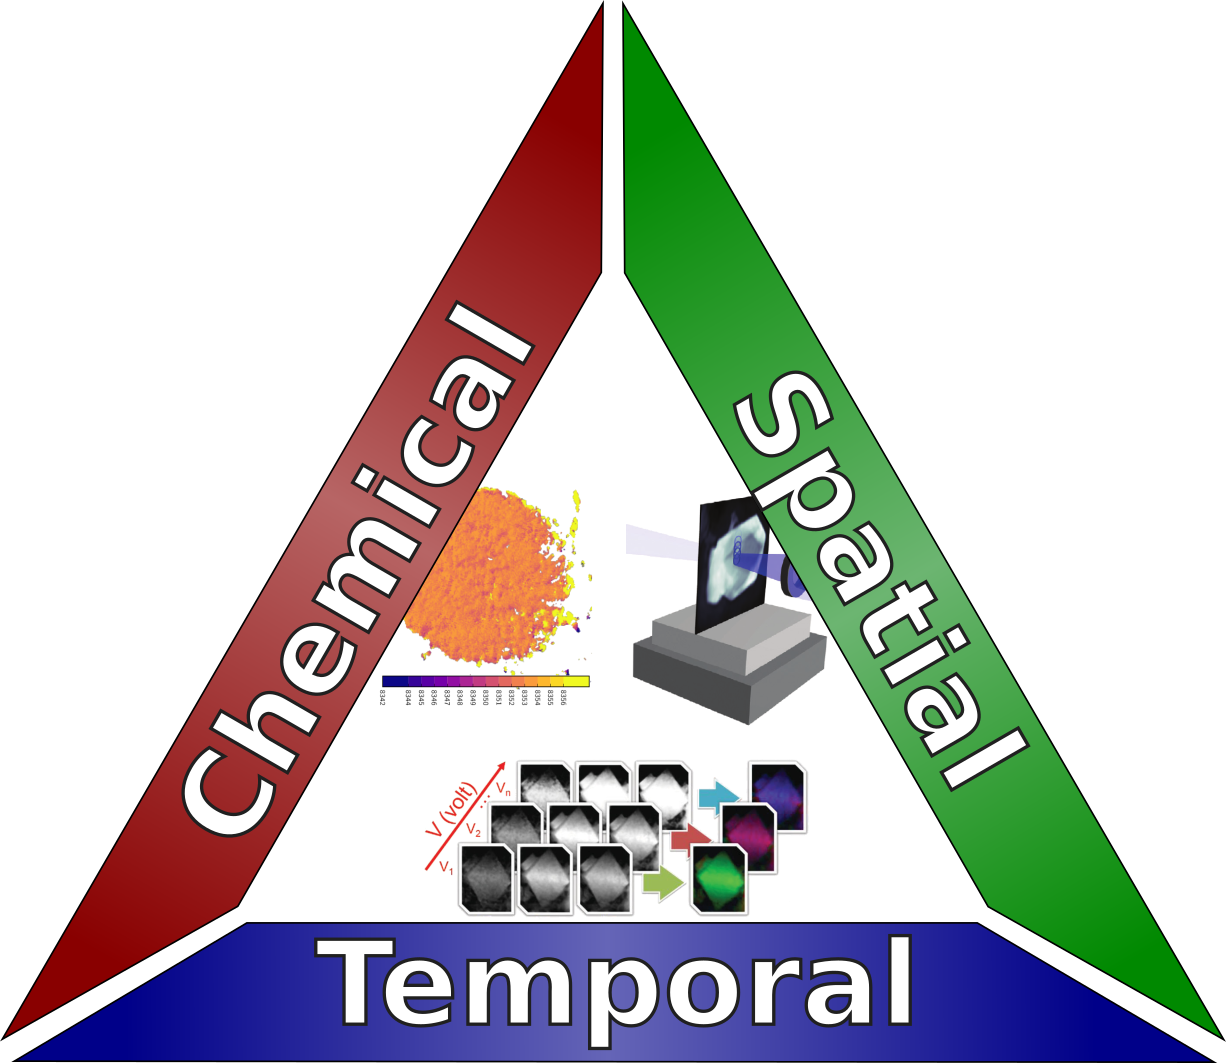
\includegraphics[width=\textwidth]{resolution-triangle.png}
  \caption{Resolution triangle, showing the trade-off between
    chemical, spatial and time resolution. Reprinted in part with
    permission from Yu et al.\ Nonequilibrium Pathways during
    Electrochemical Phase Transformations in Single Crystals Revealed
    by Dynamic Chemical Imaging at Nanoscale
    Resolution. \textit{Advanced Energy Materials} \textbf{2015},
    \textit{5}. Copyright 2014 John Wiley and Sons. Reprinted in part
    from reference\cite{shapiro2014}.}
  \label{figure:resolution-triangle}
\end{figure}

\section{The X-ray Imaging Experiment}

\subsection{X-ray Sources}

X-ray generation is possible by two different means: laboratory
sources and synchrotron facilities. The general
concept of the lab source is based on tubes under vacuum, containing a
cathode that is biased so as to generate and accelerate
electrons. These electrons collide with the metallic anode, generating
X-rays over a narrow range of wavelengths. The specific wavelengths of
the resultant X-rays are dependent on the metal used for the
anode. Common laboratory X-ray sources include the sealed X-ray tube
and rotating anode generator, which differ on the level of vacuum,
seal and the arrangement of the metallic anode\cite{guinebretiere}.

Synchrotron radiation is also generated from accelerating charged
particles, but provides higher intensity and better coherence than is
currently possible with laboratory sources. The particles,
typically electrons, are first accelerated to relativistic speeds, at
which point they enter the storage ring of the synchrotron. Beamlines
are built tangential to the storage ring so as to utilize X-ray
radiation generated when the particles are subjected to centripetal
acceleration, either through bending magnets or insertion devices,
such as wigglers and undulators. Bending magnets serve two
purposes. First, they are placed in such a way that the charged
particles in the storage ring are redirected to maintain a proper
pathway. Second, each redirection generates X-rays, which are then
used in experimental stations. Insertion devices are
specialized for generating X-rays and differ from bending magnets in
that they are straight sections of the ring that have alternating
magnetic fields. Charged particles oscillate through the device, with
each oscillation essentially equivalent to a single bending
magnet. Therefore, the generated photons can reach higher energies
than those generated by bending magnets\cite{synchrotronradiation}.

An important distinction between laboratory X-ray sources and
synchrotron sources is the nature of the X-rays produced. Synchrotron
light sources can generate X-rays at much higher intensity than
laboratory sources, which can be described in terms of flux and
brightness. Flux is representative of the number of X-ray photons that
pass a plane per unit time, typically given in photons/second. The
definition for brightness varies from author to author, however, the
National Institute of Standards and Technology (NIST) defines it as
``the radiated power per unit solid angle per unit area normal to the
[vector] direction''\cite{sesame2004}. To put it simply, brightness is
analogous to the flux, while taking into account the source size and
divergence. Another major difference between laboratory sources and
synchrotron sources is that the optics within a synchrotron create a
tunable polychromatic X-ray beam, which can subsequently be set to a
narrow energy range through the use of monochromators upstream from
the end station. In contrast, laboratory sources only produce a
limited range of X-ray energies, which is non-trivial to tune. While
some techniques fully utilize the white beam\cite{ice2009}, it is more
common to select a single desired wavelength and change it during the
experiment. The high flux, brightness and tunability renders synchrotrons as the preferred
light sources for chemical imaging.

\subsection{Methods of X-ray Microscopy}

There are two general modes of X-ray microscopy: full-field and
scanning (as illustrated in figure \ref{figure:maser2005}). The
operation of a full-field X-ray microscope is similar to a
conventional visible light microscope. In a full-field microscope, the
X-ray beam is first focused down to a few microns. This microbeam
illuminates the sample, generating a large field of view. The
resulting photons are magnified by a second set of optics before
reaching the detector.  In this mode, the limit in spatial resolution
is set by the detector pixel size and any aberrations in the
optics. This method results in large images with fine resolution in a
single shot. In contrast, a scanning microscope is based on focusing
the beam prior to illuminating the sample.  In order to collect frames
of view that are larger than the illuminated spot, the beam is
subsequently rastered over the region of interest in the sample. In
this case, the spatial resolution is determined by the combination of
beam and scanning step size. Given the different methods of operation,
it can easily be concluded that full-field imaging offers higher image
throughput than scanning imaging at the highest possible setting. On
the other hand, scanning techniques allow for higher versatility in
contrast mechanisms than in full field mode, especially when
combinations are desired.

\begin{figure}
  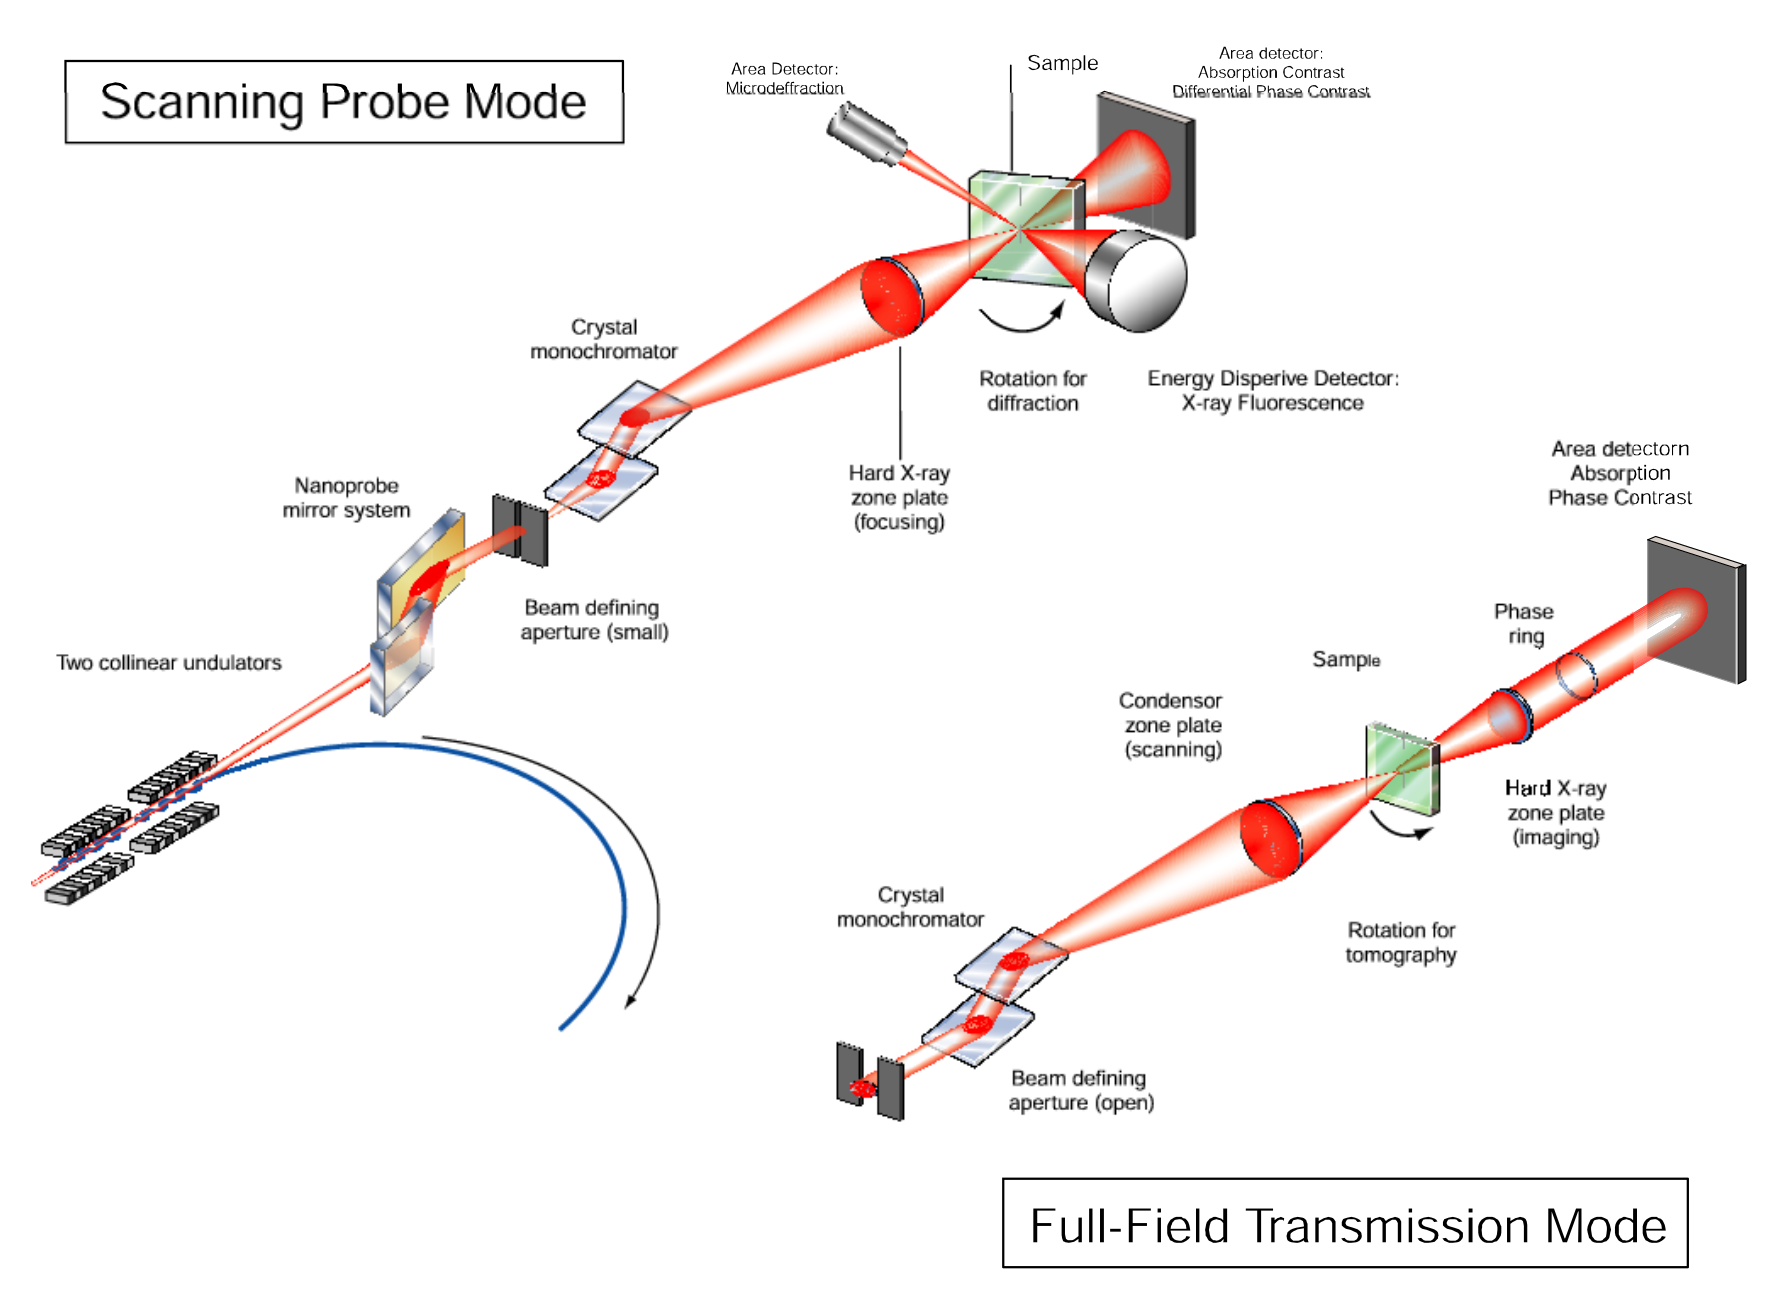
\includegraphics[width=\textwidth]{maser2005.png}
  \caption{Illustration of experimental configurations for (a)
    scanning probe and (b) full-field imaging synchrotron hard X-ray
    microscopy methods. Reprinted with permission from Maser et
    al.\ Development of a Hard X-ray Nanoprobe Beamline at the Advanced
    Photon Source. \textit{Microscopy and Microanalysis}
    \textbf{2005}, \textit{11}, 680-681. Copyright 2005 Cambridge
    University Press.}
  \label{figure:maser2005}
\end{figure}

\subsection{Tomography}

Individual images in both full-field and scanning X-ray microscopes
are generated in two spatial dimensions. However, the two techniques
offer the capability of 3D imaging using tomography. A tomographic
reconstruction is achieved by taking a series of two-dimensional
projection images while the sample is rotated over \ang{180} (ideally), followed
by conversion of these images to a three-dimensional volume. This technique is
agnostic regarding the contrast mechanism by which the two-dimensional
projections were created, meaning it can be combined with any X-ray
microscopy contrast mechanism discussed here. Provided the methodology
involves the measurement of transmitted photons, tomography allows for
the effects of sample thickness to be removed so that the intensity of
each voxel is dependent only on material composition. Since the sample
is rotating, precise alignment of the rotation axis is necessary to
keep the sample in view.

\subsection{X-ray Optics}

All the techniques discussed here require at least some level of
focusing of the X-ray beam prior to, and, in some cases, also after,
interaction with the sample. The ability to obtain images at
increasing spatial resolution is dependent on the type, sophistication
and quality of the focusing optics.

Compound refractive lenses (CRL) use several lenses in series to focus an X-ray
beam. CRLs are made of low atomic number materials to reduce X-ray
absorption\cite{lengeler1996}. Reflective
optics are used as well for X-ray focusing. First proposed by Kirkpatrick and Baez in 1948, one common setup is the use of two grazing incidence reflective mirrors that are orthogonal to
one another (KB mirrors). This setup allows for the incoming X-ray beam to be
focused in both dimensions. Both CRLs
and KB mirrors are typically used for hard X-rays\cite{kirkpatrick1948}.

Diffractive optics are an alternative option. They are predominant in
the soft X-ray regime, but are also compatible with hard X-ray
radiation. Fresnel Zone Plates (FZP) utilize several concentric rings
of alternating opaque and transparent zones, decreasing in width as a function of distance from the center. In this way, the
diffracted X-rays from the transparent sections of the optic will
undergo constructive interference, focusing to a point. The maximum amount that the beam can be focused is inversely related to the width of the outermost ring.  Multi-layer Laue Lenses (MLL) are similar to
FZPs, in that they use zones to achieve focusing. However, MLLs use
one-dimensional zones rather than rings. Because of this, they can be
synthesized using thin film deposition, which allows for smaller
thicknesses than current lithographic
techniques\cite{synchrotronradiation,lblzoneplate}.

Modern focusing optics typically limit the spatial resolution of the
measurement to roughly \SI{10}{nm}, with MLLs\cite{yan2014}. Focusing
optics have an inherent disadvantage that the resultant spatial
resolution is dependent on the optic itself. Lensless techniques
remove this restriction. Coherent diffraction patterns may be
collected and processed using an iterative reconstruction method to
produce an image. Thus, the ultimate limit resides in the wavelength
of the incoming radiation, also known as the diffraction limit,
meaning that spatial resolutions can be achieved that are smaller than
the size of the beam on the sample and the nominal resolution of the
optics. Techniques derived from this approach are further discussed
below.

\subsection{Detectors}

Detectors specific for the detection of diffracted X-rays can be
described by their geometry. Point-detectors can capture photons at
only one position at a time and are then scanned across a range of
scattering angles to acquire a one-dimensional diffraction
pattern. Line-detectors can capture a range of angles simultaneously. They produce the same one-dimensional pattern, only faster. A disadvantage of both of these
geometries is that they only retrieve a slice through the full
Debye-Scherrer rings. If only a small number of crystallites are
present, it is unlikely that any diffraction conditions will land on
this slice. For diffraction mapping techniques this is often the case,
so these detectors are unsuitable. An area detector, however, captures
a two-dimensional segment of the full pattern and so any diffraction
vectors landing within this segment will be detected. The exact range
depends on the geometry of the experimental setup and the wavelength
of radiation used: high energy X-rays cause more diffraction
conditions to be detectable in a given area. A 1-dimensional
diffraction pattern can then be obtained by integrating across the
Debye-Scherrer rings.

In full-field microscopy, the magnified X-ray image strikes a
scintillator where it is converted to visible light. The total energy
of this conversion must be conserved, so one high-energy X-ray photon
results in hundreds of low-energy visible light photons. This light is
then magnified using visible-light microscopy optics onto a detector,
usually a charge-coupled device (CCD). Any defects in the scintillator
are clearly visible in the resulting intensity images so it is
important to collect a reference frame to remove these features. For
scanning microscopy, no post-sample optics are required. Instead, a
detector measures the transmitted intensity at each raster
position. Photomultiplier tubes (PMTs) have a large collection area,
low noise and high gain, making them ideal for this application. In
some specific scanning microscopy methods, a two-dimensional
interference pattern is needed at each raster position, so a CCD
detector is used instead.

The dynamic range of the detector is an important factor to
consider. CCDs work by exposing a photo-active layer to radiation,
which then results in charge accumulation in the underlying structure,
to be read out after some time interval. If a single CCD pixel becomes
saturated before being read, any additional charge from subsequent
photons will bleed into neighboring pixels. In full-field microscopy,
this tends to be a problem in the reference images, since the maximum
intensity is larger: these areas will have artificially low values in
the resulting optical depth image. Shortening exposure time can solve
this problem, however the resulting data will have a lower
signal-to-noise ratio. A simple solution is to keep the exposure time
short and then collect and average multiple frames.

\section{Mechanisms of Chemical Contrast}

\subsection{Hyperspectral Imaging}

X-ray microscopy utilizes a multitude of contrast
mechanisms. \emph{Absorption contrast} relies on the intensity of the
X-rays that penetrate through the material being imaged. From the
physical perspective, it involves detecting changes in the amplitude
of the incoming X-ray wave after interacting with the sample. Most
commonly, the changes are detected after transmission of the X-ray
beam through the sample. Thickness and composition of the material are
two major contributing factors to the X-ray absorption. Therefore,
through the collection of one signal, both morphological and chemical
information can be generated. Since X-ray absorbance depends on
interaction with electrons, elements with higher atomic numbers have a
higher absorbance. The transmitted intensity drops exponentially with
increasing penetration length, so it is more convenient to express
this value as a logarithm of the ratio of incident radiation that is
actually transmitted; the resulting \emph{optical depth} value scales
linearly with sample thickness provided the material is
homogeneous. Two-dimensional imaging of heterogeneous samples requires
a more sophisticated interpretation since thickness and composition
both affect the absorbance. Once the X-ray energy exceeds that needed
to promote a core electron, a sharp increase in X-ray absorbance is
seen, known as an ``edge''. At these energies, core electrons are
excited either to the unbound continuum or to higher-energy unoccupied
states as allowed by selection rules. Therefore, the specific energy
value of the transition is indicative of the element and its chemical
state (eg.\ formal valence state). Each element can potentially have
several absorption edges, depending on how many core electron orbitals
it has. These edges are named based on the electron energy level they
originate from: ``K-edge'' for $n=1$, ``L-edge'' for $n=2$, ``M-edge''
for $n=3$, etc. A typical K-edge spectrum consists of two regions,
XANES (X-ray absorption near-edge structure) and EXAFS (extended X-ray
absorption fine structure). XANES provides information on oxidation
states while EXAFS provides information on local atomic structure and
neighboring atoms. In practice, collection of EXAFS data imposes data
acquisition requirements that are currently unrealistic in
spectromicroscopy. Since the oxidation state of transition metals is
of primary interest in battery materials, K-edge spectra of these
elements are a very common target for this technique. The L-edge
spectrum of an element contains information regarding the molecular
orbitals associated with its atoms, and, as a result, is also of
interest in spectromicroscopy.

\begin{figure}
  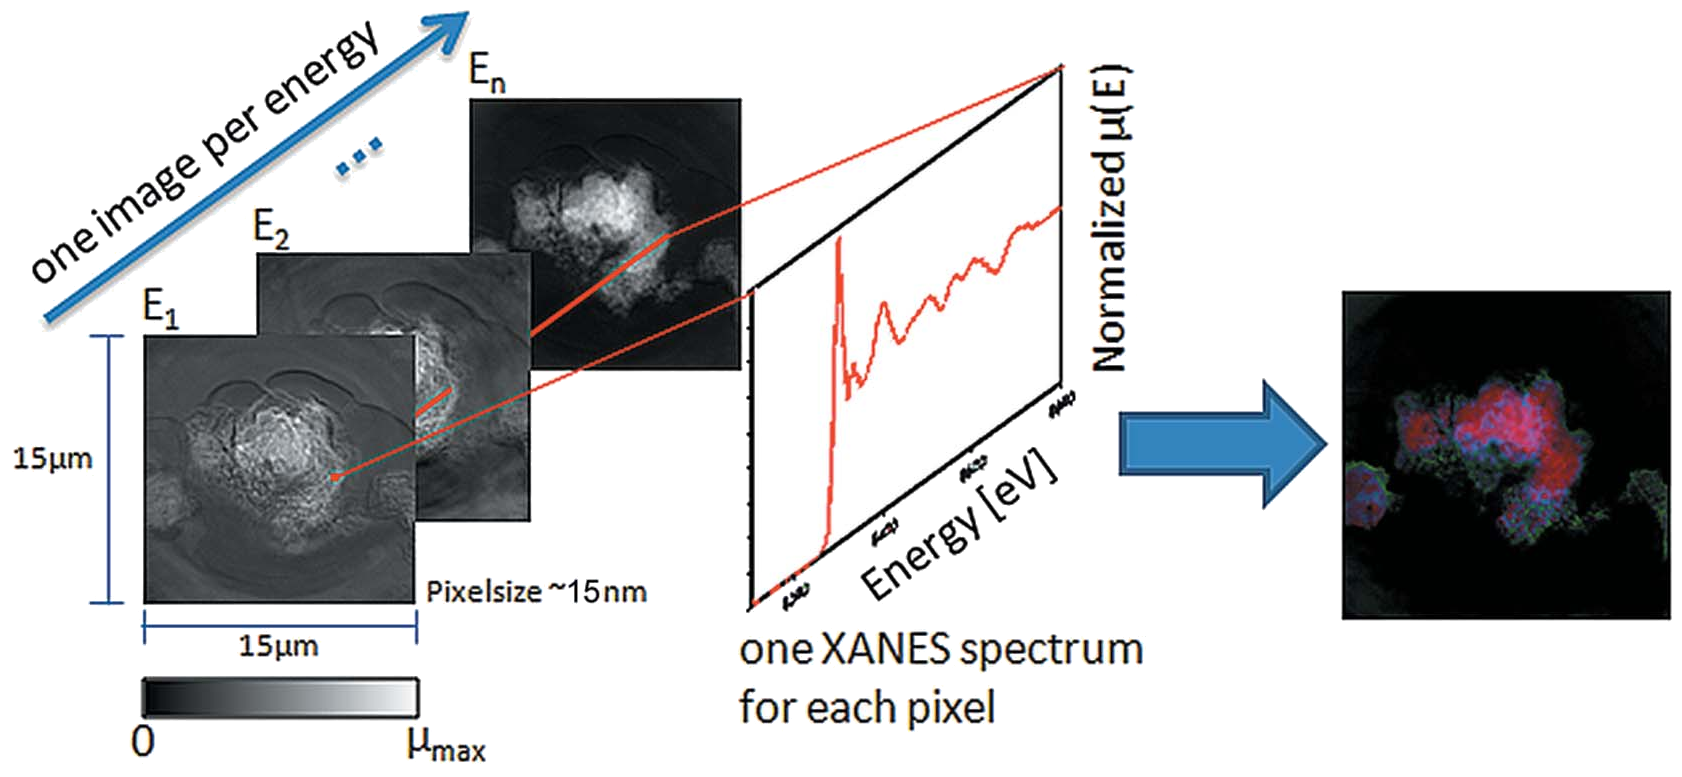
\includegraphics[width=\textwidth]{meirer2011-2.png}
  \caption{Reduction of TXM stacks to form chemical maps. A full
    spectrum is extracted for each pixel and used to calculate the
    chemical state of the material and then converted to a
    color.\cite{meirer2011} \iucr}
  \label{figure:meirer2011-2}
\end{figure}

In spectromicroscopy, whether full-field or scanning, the same
field-of-view is imaged repeatedly while the energy of the incident
beam is changed over an absorption edge of the element(s) of
interest. The resulting frame-stack provides a full absorbance and/or
phase spectrum at each pixel. These spectra are then processed into a
scientifically meaningful quantity to generate chemical maps of the
field-of-view. In order for pixel-wise spectroscopic conclusions to be
valid, it is critical that the images be properly aligned with one
another, which is rarely the case with raw data-sets. To correct for
these inconsistencies, some form of image registration is usually
necessary. The next step in the analysis involves normalization of the
spectra relative to the background optical depth. As X-ray energy
increases, the transmission of all materials increases as
well. Correcting for this effect improves the reliability of analysis
methods that involve decomposing the spectra into components of known
materials\cite{jin2015}.

Conversion of the resulting absorbance spectra to some figure of
scientific merit depends in large part on the question being addressed
by the experiment. A common goal is to map the distribution of certain
elements. This goal can be accomplished by collecting two frames per
element: one above and one below the absorption K-edge. By comparing
these ``edge-jump'' values for the elements in question, their
relative concentrations can be
calculated\cite{shieh2006}. Alternatively, generating spectroscopic
maps involves reshaping the data to give an array of spectra, each one
corresponding to a pixel in the final map. This outcome is
accomplished by ``looking through'' a frame-set along the energy
dimension and flattening along the image dimensions, as illustrated in
figure \ref{figure:meirer2011-2}. In theory, any analysis that is
performed on a bulk spectrum can be done on a single-pixel
spectrum. In practice, there are generally a lot of spectra to be
analyzed; a set of $1024\times1024$ frames contains over 1 million
spectra to be processed. This situation means that analysis cannot
rely on human intervention. If prior knowledge of the presence and
distinct spectra of multiple phases in the data-set is available,
their signals can be
decomposed\cite{wang2016,yu2015-2,shapiro2014}. If the component
spectra are not known, which is often the case, a variety of signal
processing techniques, such as \emph{independent components analysis}
(ICA)\cite{shlens2014} or \emph{Bayesian} methods\cite{knuth2005}, can
be used to approximate them and extract the relative proportions of
each component\cite{bioucas2012,duarte2014}. Care must be taken,
however, since many of these methods assume properties of the data
that are not necessarily true. \emph{Principal components analysis} is
a common alternative to ICA that has seen application in
spectromicroscopy of battery materials
\cite{shapiro2014,boesenberg2013}. Another approach involves the use
of numerical methods to directly map some property of the
spectrum. This approach is most effective if an argument can be made
that the directly calculated value correlates strongly with some
change in the properties or state of the material. For example, the
oxidation state of nickel in several layered battery cathode materials
is accompanied by a shift in the edge and whiteline positions of the
corresponding K-edge spectrum to higher energies\cite{deb2006};
extracting and mapping the whiteline position for each pixel's
spectrum can provide a map that approximates the oxidation state of
the metal and consequently the state-of-charge of the material. Care
must be taken to account for small variations in absorbance across the
two or three largest absorbance points which are not due to the
sample, but background or spurious signals.

\emph{Fluorescence contrast} is similar to X-ray absorption in that it
relies on electron excitation. The fluorescence signal, however, comes
from the subsequent light re-emission. For the element of interest,
the X-ray energy can be set just above the absorption edge. If the
incoming X-ray energy is set above the absorption edge for several
elements in a sample, they will all fluoresce at different
energies. Thus, fluorescence imaging can be advantageous over X-ray
absorption for gathering elemental distribution, especially in dilute
samples. If the energy is scanned below and through the edge,
fluorescence detectors can also be used to produce X-ray absorption
spectra, in a manner that is compatible with spectromicroscopy. This
approach was recently demonstrated in battery
materials.\cite{chueh2015}.

\subsection{Bragg Diffraction Microscopy}

Bragg X-ray diffraction (XRD) provides complementary information to
spectroscopy. Rather than observing electronic transitions, it
provides a measurement of the distance between crystalline planes
(d-space) within a material. This crystallographic information means
that unit cell parameters, atomic defects, strain and microstructural
information of the coherent domains are available. Of particular
interest in the context of this discussion is the ability to interpret
the unit cell dimensions as a given chemical composition if prior
knowledge of the system exists. In order to observe diffraction from a
material, the Bragg condition must be satisfied, in which a particular
X-ray wavelength, crystal spacing, and orientation must be met. A
conventional XRD experiment holds the X-ray wavelength constant, while
altering the incident and detected beam angles. In contrast, energy
dispersive X-ray diffraction (EDXRD) holds the orientation constant
and varies the wavelength. As a result, no goniometer is required and
the variation in wavelength can be used to profile the depth of the
sample, but extracting physical quantities from the resulting data is
less straightforward\cite{michel2005,strobridge2015}. Once a
diffraction pattern is obtained, crystallographic parameters can be
extracted and used for mapping. The data generated in Bragg
diffraction microscopy experiments can be treated very similarly to
those collected during spectromicroscopy. Each mapping position is
equivalent to a pixel in an X-ray micrograph and a series of frames
are collected at different scattering vectors, $q$. Generally, the
spatial dimensions are the slowest-changing in diffraction mapping,
whereas they are the fastest (or even simultaneous) in microscopy;
this distinction does not change the structure of the data in a
significant way. However, it does obviate the need to align each
image. Rather than a full absorbance spectrum at each location, these
experiments generate a diffractogram at each position. Theoretically,
a researcher can analyze the two-dimensional diffraction pattern at
each position; often, the 2D patterns are integrated to form the more
traditional 1D diffractograms. From here, a refinement can retrieve
crystallographic parameters, such as unit-cell dimensions, strain or
phase ratios.

\subsection{The Ultimate Frontier: The Lensless Microscope}

An alternative to imaging of absorbance and diffraction events,
\emph{phase contrast} imaging monitors the changes of the observed
phase of X-ray waves, as opposed to their amplitude, denoted by the
phase shift term, $\delta$. These changes are observed as the
thickness/density of the sample changes. In order to resolve the
observed differences in the phase shift, the detector is generally
placed far behind the sample. The distance can vary from technique to
technique; \SI{0.9}{m} has been reported for coherent diffractive
imaging (a specialized mode of phase contrast imaging described more
fully below)\cite{shpyrko2014}, while \SI{108}{cm} has been reported
for a more traditional experiment\cite{wen2014}. Phase contrast
imaging is advantageous as it is more sensitive than absorption
contrast, and can therefore utilize lower X-ray energies. Therefore,
this technique is often used to study materials that do not absorb
strongly or materials sensitive to radiation damage caused by high
energy X-rays. A drawback for some, phase contrast imaging heavily
relies upon a highly coherent X-ray source, as well as a sophisticated
detector. A full complex refractive index can be acquired using phase
contrast, by collecting data over a range of energy points. This
information will also be dependent on the electronic structure of the
sample.

A technique that uses phase contrast imaging in conjunction with Bragg
diffraction is coherent diffractive imaging (CDI). A single particle
fulfilling the Bragg condition is illuminated by a coherent X-ray beam
that is larger than the particle. The detector is placed far away from
the sample, so that it can collect fringes of the diffracted beam. An
iterative algorithm is used to reconstruct an image from the phase
information in the fringes of a three-dimensional diffraction
pattern\cite{robinson2009}.

\begin{figure}
  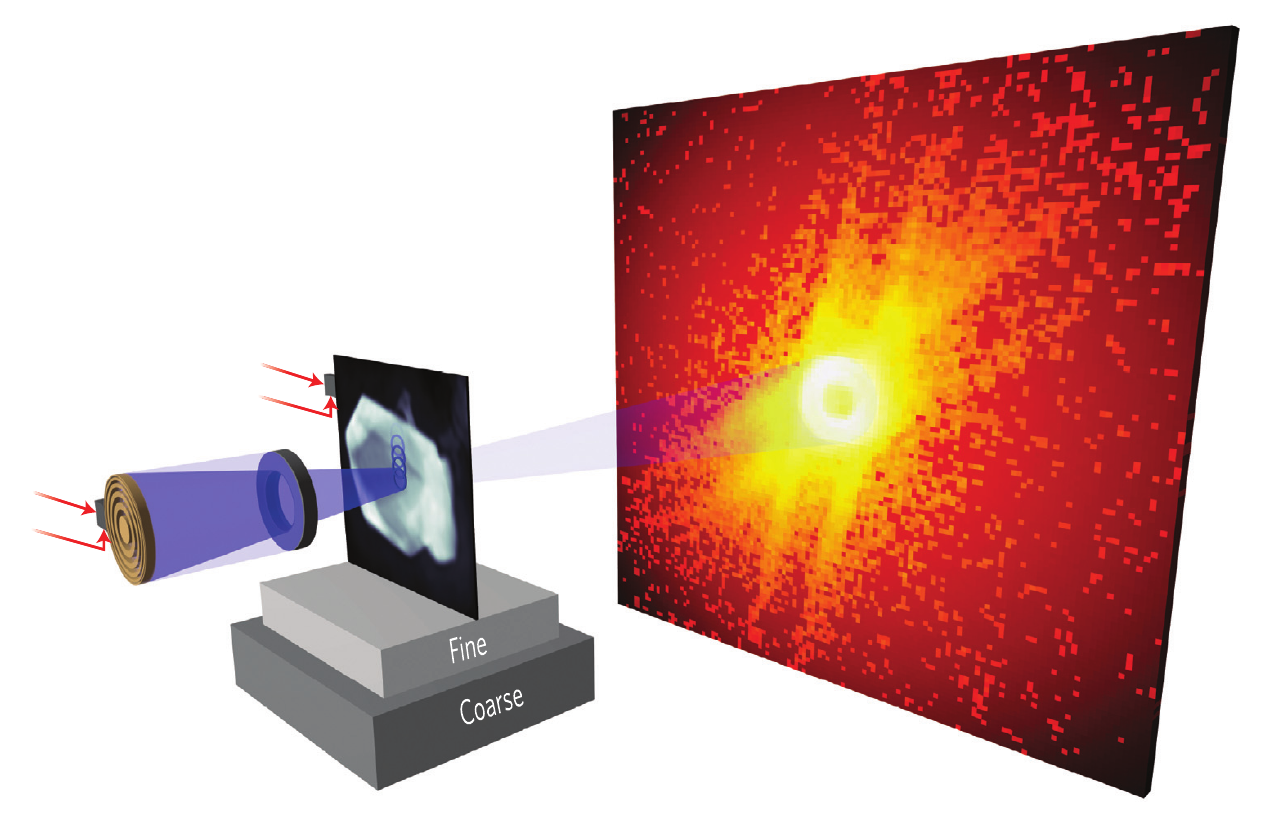
\includegraphics[width=\textwidth]{shapiro2014.png}
  \caption{Schematic of soft X-ray ptychographic microscope. An
    incoming X-ray beam is focused onto the sample by a zone plate and
    order sorting aperture. The coherent diffraction pattern is
    collected by a CCD\cite{shapiro2014}.}
  \label{figure:shapiro2014}
\end{figure}

Ptychography is another lensless technique which also relies on
collecting the full diffraction pattern using coherent
diffraction. Unlike CDI, this is a scanning technique; small spots are
collected in such a fashion that they spatially overlap on the
sample. Similar to CDI, ptychography utilizes an iterative algorithm
to reconstruct an image from the diffraction patterns. A random object
image is first generated. For each scanning position, a Fourier
transform is performed on the object and is convolved by the
illumination probe. The real component is replaced by the recorded
interference pattern and an inverse Fourier transform is then done to
recover an improved object. This procedure is carried out for each
scanning position and repeated until a solution converges. As a
result, the ultimate spatial resolution is, to a large extent,
independent from the size of the beam used to collect the overlapping
patterns. In other words, as a lensless technique, the process of
generation of images does not suffer from lens aberration and thus
allows for very high spatial resolution approaching the diffraction
limit, under \SI{10}{nm} in some cases. Artifacts from the
reconstruction process sometimes manifest as high frequency bands
alongside sharp edges in the specimen. Since this technique is driven
by an interference pattern, the best reconstructions are obtained from
strongly scattering materials. Ptychography has also been performed in
tomographic mode\cite{venkatakrishnan2016}, but this methodological
area is still in its infancy. As an added bonus, the reconstruction
produces both the real and imaginary components of the object
image. By comparison to an area with no material, the fully complex
refractive index can be calculated. Exploiting the complex-valued
nature of this technique is a relatively unexplored area.

\subsection{Visualization and Colormaps}

Turning a large data-set into a two-dimensional image is a task that
becomes more challenging as the number of dimensions increases. For
applications with two spatial dimensions, map images are generated by
data-reduction as described in the preceding sections. The
relationship between values and colors is known as a ``colormap'' or
``lookup table''. The choice of colormap can have subtle effects on
how the data are interpreted. In general, human vision associates the
brightness of a color with the value it represents, regardless of its
hue. Therefore, an effective colormap translates high values to
high-brightness colors and low values to low-brightness
colors. Rainbow colormaps, such as \emph{jet}, do not meet this
criterion and should be avoided for representing sequential data. Jet
contains bands of high and low brightness that are perceived as sharp
gradients in the data that do not actually exist. Perceptually uniform
colormaps, such as \emph{viridis} for Matplotlib and \emph{parula} for
Matlab, are designed to avoid this problem. Additionally, viridis was
tested against color blindness and ensures that data display properly
to people in this category.

Projecting data with three spatial dimensions onto a two-dimensional
canvas can be done with any one of several visualization
tools. Typically, certain features in the data are of interest, such
as internal fractures within particles or the distribution of certain
elements. Successful visualization usually requires additional
analysis steps that identify and highlight these features while making
the surrounding material partially transparent. Avizo (FEI) is a
popular commercial software package specifically designed to work with
tomography data: it contains a number of filters that allow the data
analysis to be performed within one piece of software. An additional
Avizo package can be purchased that allows it to handle data-sets that
do not fit entirely into main memory, which is often the case for
tomography. An alternative is
\href{http://www.paraview.org/}{Paraview} (Kitware Inc. and Los Alamos
National Lab), a general purpose visualization platform that is highly
extensible, allowing python plugins to be run from within the
application. Paraview has the additional benefit of being free and
open source. For quick inspection of tomographic slices, ImageJ
provides the
\href{https://imagej.nih.gov/ij/plugins/volume-viewer.html}{Volume
  Viewer plugin} (included in the \href{http://imagej.net/Fiji}{FIJI
  distribution}), which is more straight-forward to use than either
Avizo or Paraview, but has fewer features.

\section{Ex situ \latin{versus} operando}

To a large extent, electrochemistry is most interesting when away from
equilibrium. As electrochemical devices, batteries are useful during
operation, which is inherently under kinetic control. While the
kinetic states are determined by the thermodynamics of the system,
metastability is more prominent under electrochemical conditions than
in other classical chemical environments, such as high
temperatures. This prominence also implies that the probability of
producing kinetic states that are only weakly metastable is high. In
fact, the problem of self-discharge, common in certain batteries, is
precisely the product of equilibration of a metastable charged
state. As a consequence of the pervasive kinetic control, ex situ
measurements, which rely on harvesting samples from a cell at a
desired chemical state, introduce uncertainty when the goal is to
describe relevant states under working conditions. Nonetheless, if
caution is applied, and due to their simplicity, these measurements
can still provide valuable guidance\cite{yu2015-2}, mainly because
they do not critically suffer from constraints in measurement time
and, thus, can result in the highest data quality. Ultimately,
operando measurements of battery reactions are preferred because of
the growing body of evidence showing that there are many cases where
the state within an operating battery is different from what is
observed once the cell is disassembled\cite{liu2014, lim2016},
especially when high rates are employed. For this reason, researchers
developing novel methods of imaging should have motivation to enter a
path that results in means to operando analysis. At this point, given
certain confusion in the field, it is worth clarifying that we
consider operando measurements to be a small subset of in situ
science. The condition sine qua non for an operando experiment is that
the cell is not stopped to collect data unless the goal is
specifically to measure equilibration phenomena.

While operando measurements are preferred and should be pursued, they
can present several challenges of varying degrees of difficulty. The
setup must allow photons to pass through both the sample and apparatus
with very little disturbance to the signal from the apparatus
itself. First and foremost, X-ray absorbing materials have to be
minimized in order to ensure sufficient signal reaches the
detector. Ideally, supporting materials containing heavier elements
should be removed, or made sufficiently thin so as to minimize their
effects. Another challenge is avoiding X-ray induced damage to
supporting materials, such as the polymer binder often used in the
construction of cathodes. Maintaining adequate stack pressure may also
be important, depending on the nature of the
experiment\cite{borkiewicz2015}. Additionally, the possibility of
deleterious effects of X-ray exposure on the behavior of cathode
materials is not completely understood. One possibility is to use very
high energy X-rays, which can penetrate the casing
material\cite{lin2013} and are less damaging. This strategy is valid
for some diffraction experiments, but cannot be applied to
spectroscopic imaging since specific energies at which the X-ray beam
is absorbed are required.

In situations where high-energy X-rays are not possible, a transparent
window is necessary. Beryllium is a typical choice, but its use
introduces stringent handling requirements due to its high toxicity,
especially in the dispersible form that is generated, for instance,
during machining. It also oxidizes relatively easily, making it
unsuitable for high-voltage battery applications. Silicon nitride is
an appealing option since it can be purchased commercially in
prefabricated windows down to tens of nanometers in thickness. At
these thicknesses, it also does not have any noticeable morphological
features, making it suitable for X-ray microscopy techniques. However,
they are very fragile due to their thickness. Polyimide (Kapton) film
has found widespread use in operando diffraction experiments, despite
the fact that it also introduces an amorphous contribution to
diffraction patterns. It has relatively high transmissivity, is easy
to fabricate and is chemically inert. Unfortunately, it cannot ensure
a complete seal and, like many other plastics, it often contains
filler particles which are heavy enough to become visible in a
microscopy experiment, interfering with observations and, thus,
rendering it unsuitable. Amorphous carbon can also be used. A large
advantage here is its electrical conductivity, which eliminates issues
of electrochemical inactivity of the material behind the window. Since
it is made entirely of carbon, it also interacts only very weakly with
X-rays, so it induces minimal signal attenuation. However, it is
difficult to fabricate, and can react under certain conditions, such
as at very high potentials or against lithium metal. The AMPIX
electrochemical cell, developed by Argonne National Laboratory, is an
example of a cell with amorphous carbon windows that fits the
requirements of an operando X-ray experiment. The cell design ensures
good stack pressure as well as electrical conductivity, closely
mirroring coin cell
conditions\cite{borkiewicz2012,borkiewicz2015}. Even more
sophisticated cells are needed when using low energy, soft X-rays,
where the sample volume must be small to avoid excessive absorption of
the signal by the sample. In this case, designs that rely on
microfabrication have recently been demonstrated\cite{lim2016}.

\begin{figure}
  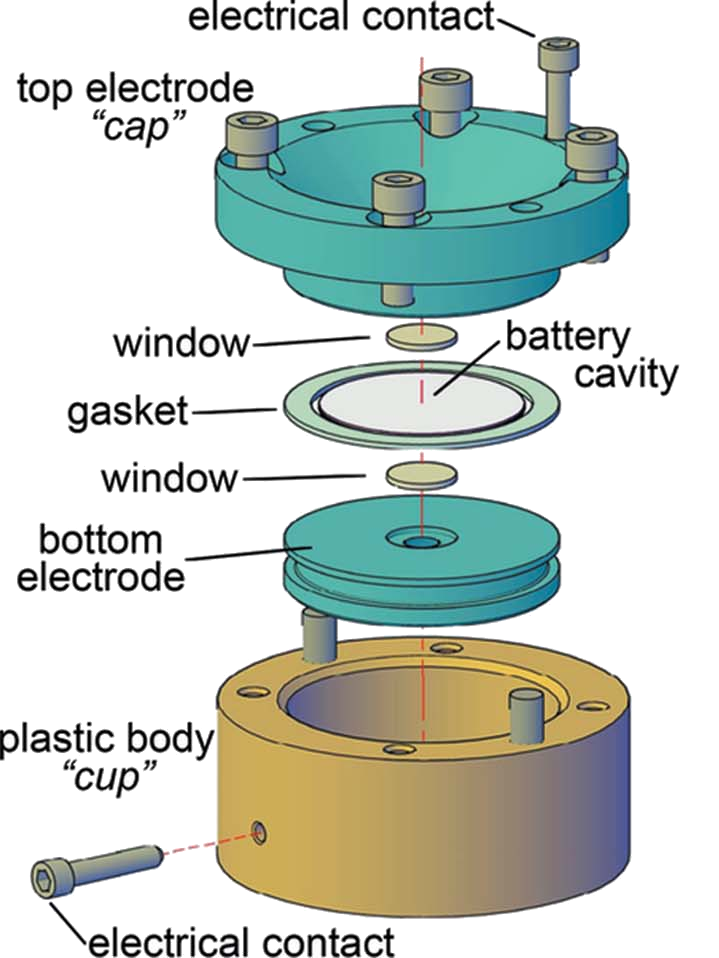
\includegraphics[width=\textwidth]{ampix.png}
  \caption{Schematic of AMPIX electrochemical cell.\cite{borkiewicz2012} \iucr}
  \label{figure:ampix}
\end{figure}

Operando measurements create the most severe challenges to an imaging
experiment when considering the three scales of resolution above,
namely spatial, chemical and temporal. Many battery reactions span
several hours, but the need to build a reaction pathway means that it
is desirable to collect at least 5 data points during the
reaction. This goal imposes restrictions on the time available to
complete an image containing the desired chemical information, at the
desired level of spatial resolution. Unfortunately, all modes of
chemical contrast require collecting multiple frames for the same
reaction state to reconstruct a map of the species present in the
field view. Using XANES microscopy as an example, chemical resolution
is achieved by collecting frames at a large number of energies, with
the limit being set by the precision of the upstream optics. In the
particular case of scanning techniques, spatial resolution requires
the use of the smallest possible step size to raster the field of
view, meaning that a similar trade-off emerges in that the acquisition
time is directly affected by this parameter. Additionally, increasing
the collection time for each frame will improve the signal-to-noise
ratio and improve the accuracy of the data, again at the expense of
longer acquisition times for a full frame-set. In practice, the most
common choice is to minimize the number of points to obtain some level
of chemical resolution in the individual frame-set, whether scanning
energy (spectroscopy) or a beam-sample-detector angle
(diffraction). This approach strongly relies on prior knowledge of the
chemical species involved during the reaction, so that energies or
angles are chosen at which signals between these species differ the
most. Such prior knowledge is typically acquired through XAS or XRD
measurements of the bulk average, as opposed to spatially resolved
regions. In the case of the spectroscopy of transition metal species,
a change of one unit in the formal oxidation state translates into a
displacement of the signals of a few electron-volts, which renders the
method viable. Challenges arise when the changes between species are
small, for instance, when compounds exist at redox states intermediate
between end members. The strategy also inherently lends itself to
misinterpretation if previously unknown or unexpected states form in
the measurement, especially if they are related to the known, expected
species. The local character of an imaging measurement means that the
limit of detection of minority species increases with respect to a
data set gathered from the bulk average, especially if they
accumulated in specific regions of the image. All in all, it is
important to be aware of the compromises made to avoid over-analyzing
data. Since the field of X-ray imaging is vibrant and constantly
pushing the boundaries in resolution, it is likely that these
limitations will be alleviated with time, creating exciting
opportunities for rich insight into battery operating conditions.

\section{Applications of X-Ray Imaging to Problems in Battery Research}

In this section, we describe case studies that highlight the power and
versatility of X-ray imaging to elucidate phenomena occurring in
battery materials. As a result, this section is not meant to be
exhaustive. We mostly focus on examples of electrode materials
containing transition metals, as they are the most pervasive in the
literature. Many relevant cathode materials are not discussed
(eg.\ Zinc-air) because the imaging aspects of the research are already
covered by other examples. The specifics of each material are not
discussed beyond their chemical identity and a brief mention of the
insight gained by imaging. For an extensive discussion of the current
body of knowledge of electrochemical reactions in the battery
materials discussed here, the reader is referred again to reviews
existing in the literature\cite{whittingham2014,
  balogun2016}. Selected applications are grouped by contrast
mechanism. X-ray imaging at one or two energies close to an
absorption edge can be used to elucidate morphology or elemental
distribution respectively. While these approaches can provide valuable
information, chemical (XAS) or structural (XRD/CDI) imaging generally
provides a richer and more insightful data-set; consequently, many more
examples of novel applications are available for these two categories.

\subsection{Morphology}

%% Intro to general morphology
Absorption imaging at a single X-ray energy provides a direct look at
the internal morphology of the material. The short acquisition times
and relatively straightforward technical requirements mean that high
temporal resolutions can be achieved. Paul Shearing \emph{et
  al.}\ used full-field X-ray microscopy to characterize thermal
runaway in an 18650 cell with a time resolution of
\SI{800}{\micro\second}\cite{shearing2015}. This represents one
extreme of the resolution triangle, where no chemical contrast is
provided and spatial information is limited to two-dimensional
projections. The result was a high frame-rate movie showing the
initial distortion of electrode layers followed by gas formation and
finally the catastrophic structural failure of the cell.

%% Intro to 3D morphology
Tomography solves a common problem where interpretation of two
dimensional imaging data is confounded by the fact that the measured
intensity at each position is a projection through the entire
specimen. Operando tomography will be a key technique in achieving a
thorough understanding of battery material mechanisms. Tomographic
morphology imaging can even be achieved with laboratory X-ray
microscopes\cite{shearing2014-2}. Despite the lack of direct chemical
information, this technique can illuminate details of the underlying
mechanism, as illustrated by some recent publications. In conversion
reactions, mixtures of relatively heavy metallic particles and
\ce{Li2O} are formed\cite{cabana2010-2}. Since the differences in
attenuation coefficients of the different species are quite large,
quantification of changes in contrast in the image can be used to
create pseudo-chemical maps. This approach is relatively fast, since
data collection occurs at only one X-ray energy. This idea was first
exploited by Ebner et al.\ to study the reduction of tin oxide. A
core-shell mechanism was observed as well as detailed information
about crack initiation and growth. They also compared particle-level
volume changes and their relationship to the expansion of the
electrode as a whole. They found that the particles expand beyond the
tolerance of the supporting matrix, which has implications for the
reversibility of the reaction\cite{ebner2013}. A similar approach to
the analysis of individual tin oxide particles during the first two
charge-discharge cycles showed significant fracturing and
pulverization, with an accompanying loss in reversible
capacity\cite{wang2014-2}. This single-energy approach to acquiring
chemical contrast is only valid for three-dimensional imaging since in
two-dimensions the intensity of a given pixel is heavily influenced by
the thickness of the sample at that point. Another limitation is that
majority of reactions of interest in batteries involve compounds that
do not show significant differences in attenuation coefficient. In
these cases, advanced tomographic techniques are needed, as discussed
below. Even in intercalation materials, where optical density does not
change significantly with charge-state, morphology can still reveal
useful information regarding the electrode performance. For example,
the novel use of a heat-transfer model to extract tortuosity and
porosity data from three dimensional electrode volumes revealed
significant anisotropy and heterogeneity in the pore structure, with
implications for modeling electrode behavior\cite{shearing2014}.

\subsection{Elemental Distribution}
%% Elemental distribution examples
Several experiments highlight the ability of X-ray imaging to track
the distributions of specific elements in battery materials. Migration
of transition metals after one cycle was seen by X-ray absorption
tomography\cite{yang2014-2}. Specifically, the authors discovered
depletion of the transition metals at the surface of the particle,
accompanied by manganese segregation. Another example used this
technique to track transition metal distribution across multiple
cycles in a particle of mixed transition metal oxide
\ce{LiNi_{0.4}Mn_{0.4}Co_{0.2}O_2}\cite{lin2016}. The authors showed
an excess of manganese and a depletion of cobalt and nickel at the
surface of the particles when using specially designed materials. It
is known that an irreversible conversion of nickel to a reduced
rock-salt phase occurs at the surfaces in these materials. This low
cobalt/nickel material shows a subsequent improvement in high-voltage
electrochemical cycling performance.

\subsection{Chemical Imaging}

\hl{RFC: Does this intro section read well with the ``methods'' description?}

% Chemical imaging introduction
Many of the materials used for battery cathode materials do not show
significant changes in absorbance between the various states
encountered during operation, limiting the scope of the morphological
and elemental-distribution techniques. X-ray absorbance spectroscopy
provides a direct measure of the chemical state of individual
elements. Therefore, it can be used to track the oxidation state of
the electrochemically active species. This approach is not limited to
a specific technique: it has proven insightful using hard and soft
X-rays, K and L absorbance edges, full-field and scanning microscopes,
and in two-dimensional and tomographic imaging modes.

Hard X-ray full-field microscopy has seen rather broad applicability
to questions in battery research. It has effectively been demonstrated
to locate delithiation domains in olivine-type \ce{LiFePO4}
microcrystals, and subsequent morphological events, such as fracture
were identified\cite{boesenberg2013}. However, the spatial resolution
of a hard TXM, $\sim$\SI{30}{nm}, did not allow for a specific
correlation between chemical domains and fracture points. To achieve
this knowledge, soft X-ray absorption spectroscopy coupled with
ptychographic microscopy was required in order to gather information
at the highest spatial resolution possible today. Yu et
al.\ investigated how crystal size impacts the transformation of
\ce{LiFePO4} to \ce{FePO4}\cite{yu2015-2}. Chemical maps were
successfully produced for particles ranging from <\SI{100}{nm} to
several microns in length. The high spatial resolution achieved in
these ptychography measurements, $\sim$\SI{10}{nm}, finally revealed
the correlation between chemical states and physical artifacts, such
as cracks. Indeed, comparison of ptychographic imaging with
conventional scanning spectromicroscopy highlights the increase in the
sharpness of the images, which makes spatial correlation
possible. Panels a and b of figure \ref{figure:shapiro2014-2}
show the extent of improvement\cite{shapiro2014}. The work
demonstrated that reducing the size of \ce{LiFePO4} particles resulted
in less extensive fracturing while the distribution of reaction
products was very similar, which was taken as an indication of the
superior electrochemical performance from \ce{LiFePO4}
nanoparticles\cite{yu2015-2}.

\begin{figure}
  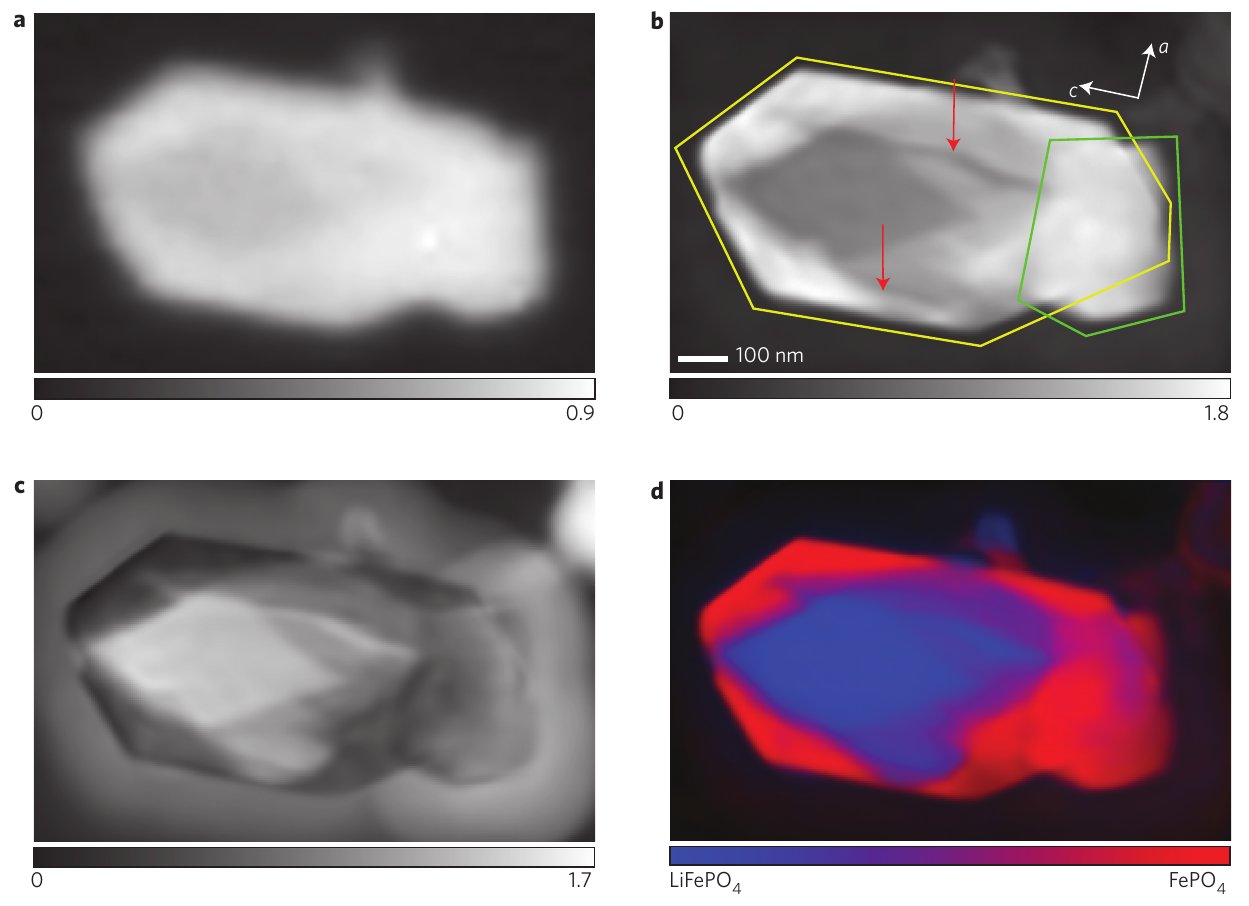
\includegraphics[width=\textwidth]{shapiro2014-2.png}
  \caption{(a), (b) X-ray microscopy of partially delithiated
    LiFePO4. Optical density maps from STXM (a) and ptychography (b)
    at \SI{710}{eV}, showing maximum absorption contrast between the end
    members. The spatial resolution of the STXM is not adequate to
    visualize the presence of multiple particles, which are outlined
    in the ptychographic image, and cracks along the crystallographic
    c axis, which are indicated by red arrows (the a and c
    crystallographic axes are indicated by white arrows; the b axis is
    parallel to the X-ray transmission). (c) Phase of the
    ptychographic reconstruction at \SI{709.2}{eV}, showing maximum relative
    phase shift between the end members. The halo around the particle
    is carbon contamination. (d) Colorized composition map calculated
    by principal component analysis, clustering and singular value
    decomposition of the full complex refractive index.\cite{shapiro2014}}
  \label{figure:shapiro2014-2}
\end{figure}

% Ex-situ XANES TXM Tomography of NiO (Cabana/Meirer paper)
Combining tomography and XANES microscopy generates a very rich
data-set that provides a window into the chemical environment at every
point in the specimen. Meirer et al.\ used 3D XANES to probe the
conversion of NiO to Ni metal in a discharged battery
cathode\cite{meirer2011}. By comparing the spectra in a sample where
the transformation was only 50\% complete to the spectra of known
reference materials, they assigned each voxel (3D pixel) to either
\ce{NiO}, \ce{Ni} metal or a 50:50 mixture of the two. Additionally,
they analyzed virtual slices through the three-dimensional particle to
determine how the chemical states were distributed. They found
significant inhomogeneities across the particle that depended on its
size, as well as evidence of fracturing caused by volume expansion
during the reaction. In this case, fracture was revealed as the
enabler of the phase progression into the particle, which critically
relies on microstructural formatting to reach completion.

\begin{figure}
  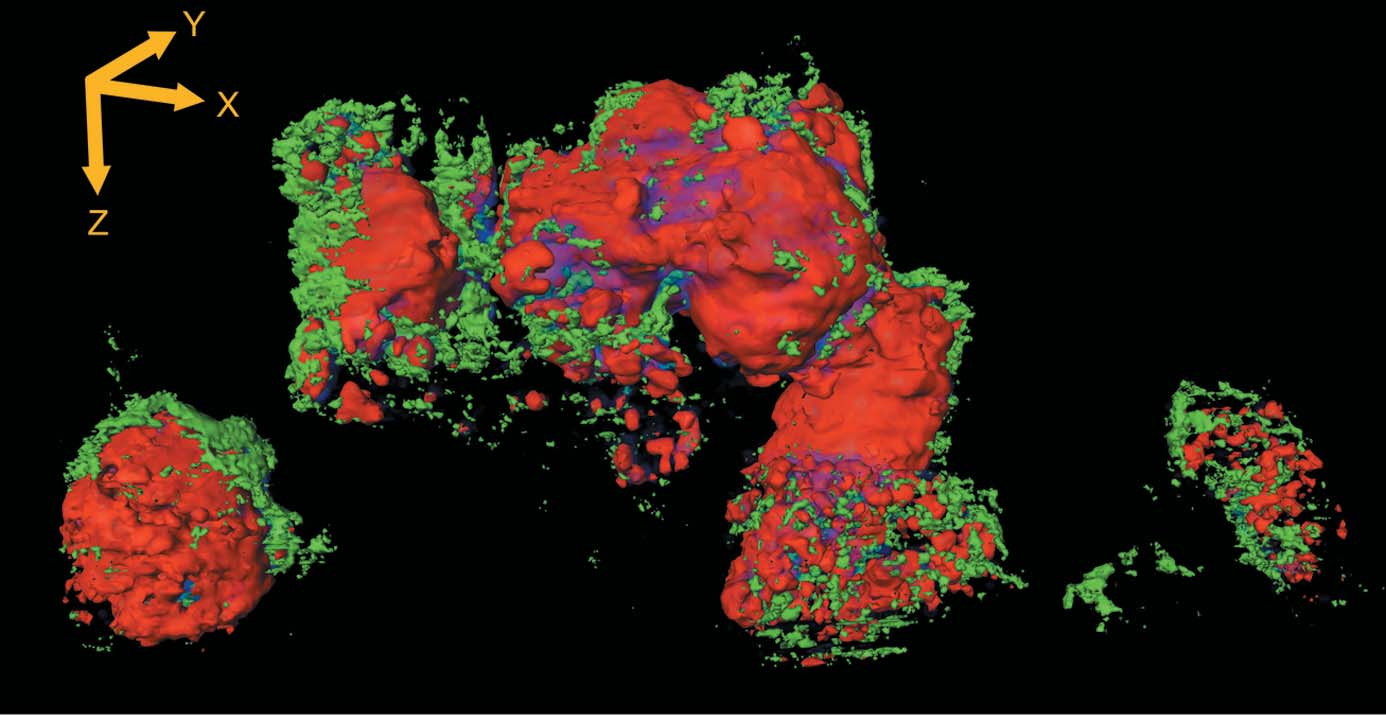
\includegraphics[width=\textwidth]{meirer2011.png}
  \caption{Reconstructed three-dimensional XANES tomography
    perspective rendering of three-dimensional data set of \ce{NiO}
    cathode.\cite{meirer2011} \iucr}
  \label{figure:meirer2011}
\end{figure}

% Operando TXM Cu-O K-edge XANES
Performing these types of measurements operando has the ability to
provide insights that are not available with other techniques. The
first demonstration of operando X-ray spectromicroscopy using a
full-field technique involved the study of the reduction of CuO
particles inside a coin-cell modified with Kapton
windows\cite{wang2013}. A distinct shell of reduced copper metal was
seen surrounded by an unreacted \ce{CuO} core, along with an
intermediate \ce{Cu2O} phase. A further iteration of this coin-cell
design was developed by Yu et al.\ and used to study \ce{LiMn2O4}
spinel crystals. In order to improve resolution across the board, the
emphasis in the design was placed on minimizing the thickness of
absorbing materials, such as aluminum, and, for instance, it relied on
\SI{1}{\micro\meter} thick silicon nitride windows. The design was
applied to the study of the transformation \ce{Li2Mn2O4}
$\rightleftharpoons$ \ce{LiMn2O4} $\rightleftharpoons$
\ce{Mn2O4}\cite{ohzuku1990}. During the experiment, the authors found
significant local effects in the oxidation of the particles, wherein
oxidized \ce{LiMn2O4} regions formed and propagated through the
crystal. Additionally, a reduced tetragonal \ce{Li2Mn2O4} phase
persisted at potentials well above its predicted stability, according
to the phase diagram, leading to a non-equilibrium coexistence with
highly oxidized phases. These observations would probably not have
been possible under ex situ conditions, where the chemical states are
expected to equilibrate. At higher potentials, several cracks in the
crystals were seen that correlated with preferential oxidation to the
fully delithiated \ce{Mn2O4} phase, as seen in figure
\ref{figure:yu2015}. The authors speculated that these cracks provide
additional, fresh interfaces to facilitate phase
transformation\cite{yu2015}.

\begin{figure}
  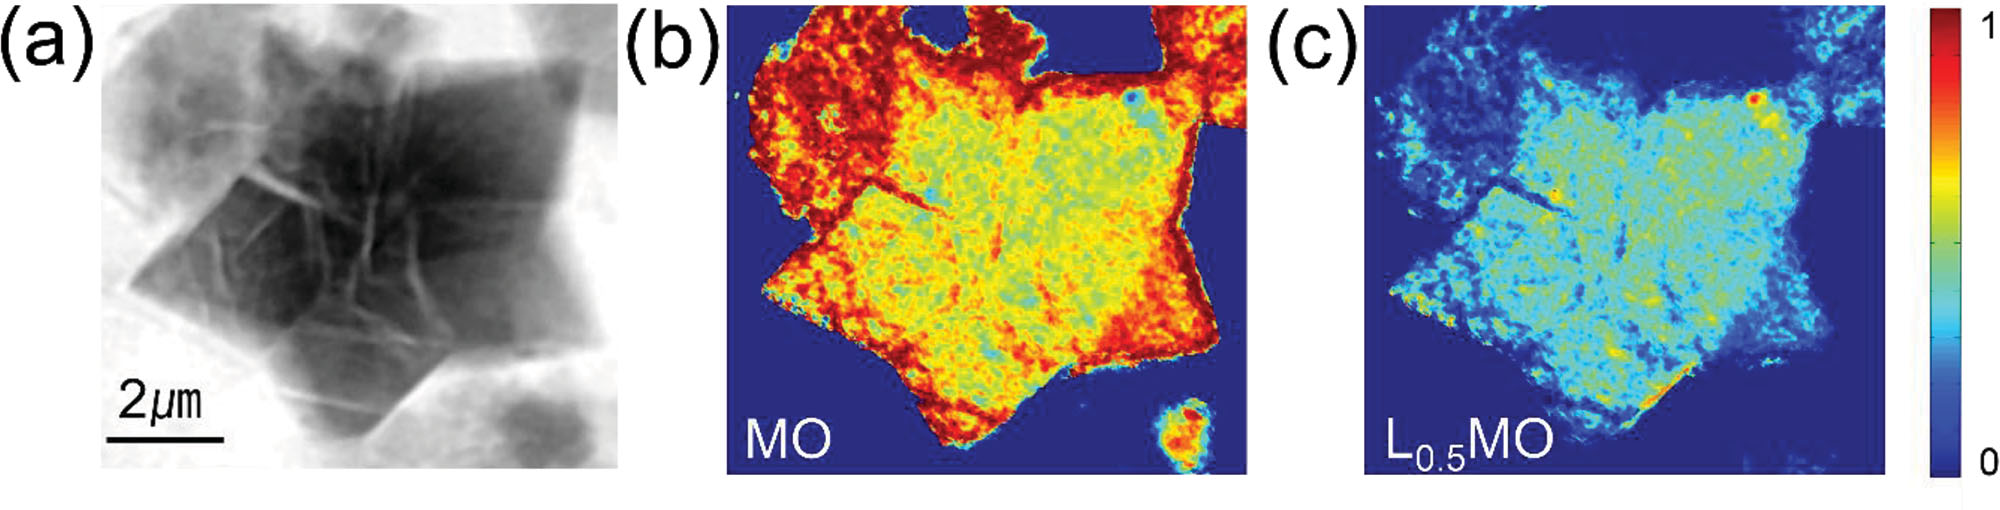
\includegraphics[width=\textwidth]{yu2015}
  \caption{Preferential growth of \ce{Mn2O4} along cracks at
    \SI{4.09}{V}. (a) Inverted optical density image collected at
    \SI{6700}{eV}. Heat maps where color contrast scales with the
    ratio of spectral standards of (b) \ce{Mn2O4} and (c)
    \ce{Li_{0.5}Mn2O4} in each pixel. Reprinted with permission from
    Yu et al.\ Nonequilibrium Pathways during Electrochemical Phase
    Transformations in Single Crystals Revealed by Dynamic Chemical
    Imaging at Nanoscale Resolution. \textit{Advanced Energy
      Materials} \textbf{2015}, \textit{5}. Copyright 2014 John Wiley
    and Sons.}
  \label{figure:yu2015}
\end{figure}

Several other recent examples of operando TXM are worth
highlighting. A study of \ce{LiFePO4} provided details about the phase
propagation mechanism and revealed inhomogeneities in the distribution
of oxidized materials between multiple particles\cite{wang2014}. Li et
al.\ studied \ce{FeF3} and showed that the capacity loss seen in this
material is due to incomplete conversion from \ce{Fe} to \ce{Fe3+}
during charging\cite{jin2015}. Another example further elucidates the
role of oxygen species in lithium-air batteries. Olivares et
al.\ looked at the formation of surface barriers, similar to the
solid-electrolyte interface, on a carbon substrate. By examining the
oxygen K-edge, they showed a relationship between particle morphology
and the preference for forming carbonate, peroxide, and superoxide
species\cite{olivares2015}. The authors argued that the reactive and
short-lived nature of some of these oxygen species ensures that
meaningful results cannot be obtained without operando measurements.

% Soft XAS  of LFP
Thanks to advances in the design of operando cells brought about by
microfluidics, scanning TXM using soft X-rays has been recently
demonstrated, and used to probe the spatial dynamics of \ce{LiFePO4}
particles\cite{lim2016}. The authors were able to collect chemical
images at a variety of rates while gathering reliable electrochemical
data. Linear combination fitting was used to create maps of lithiated
and delithiated material. It was found that the pathways upon
lithiation and delithiation were strikingly different depending on the
conditions of cycling. Thanks to the quality of the data, the authors
were also able to extract the current density for actively
(de)intercalating pixels. They found a strong dependence of the
exchange current density ($j_0$) and the degree of lithiation ($x$ in
\ce{Li_xFePO4}), as shown in figure
\ref{figure:lim2016}. Heterogeneities initially caused by other
sources are then amplified by this positive feedback mechanism during
lithiation and suppressed during delithiation.

\begin{figure}
  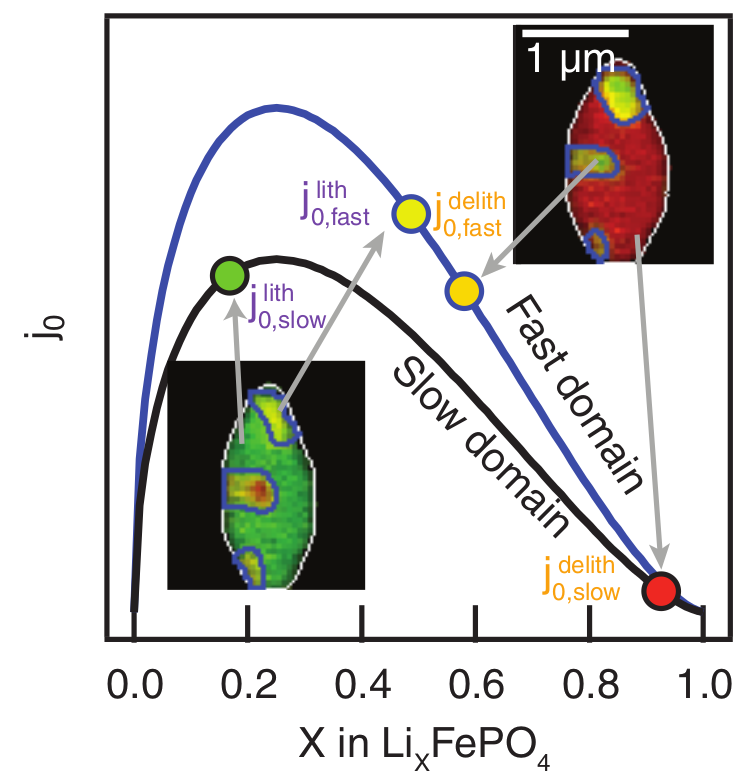
\includegraphics[width=\textwidth]{lim2016.png}
  \caption{Relationship between measured exchange current density and
    degree of (de)lithiation. Because the skewed $j_0$ peaks at $x
    \approx 0.25$, the value of $j_0$ for the fast domains is several
    times that of $j_0$ for the slow domains during delithiation, but
    the two quantities are comparable during lithiation. From Lim,
    J. et al.\ Origin and hysteresis of lithium compositional
    spatiodynamics within battery primary particles. \textit{Science}
    \textbf{2016}, \textit{353}, 566-571. Reprinted with permissions
    from AAAS.}
  \label{figure:lim2016}
\end{figure}

The only available example of operando chemical imaging in
three-dimensions highlights the challenge of interpreting projection
images directly. Wang et al.\ collected a 46-point spectrum across the
iron K-edge of a \ce{LiFePO4} cathode particle and developed a run-out
correction system to enable automated tomography. In order to
accommodate the significant overhead in time required to acquire 2D
images at different energies and angles, the battery was charged
extremely slowly (10-100 times slower than would be
realistic). Nonetheless, the insight collected was noteworthy, with
the advent of a clear core-shell structure, as shown in figure
\ref{figure:wang2016}. When considering two-dimensional projections
from only one angle, it appeared as though a mixed state existed
between the lithiated and delithiated material. Tomographic
reconstruction revealed this mixed state to be an artifact of the
projection process, as it is not present anywhere in the particle\cite{wang2016}.

\begin{figure}
  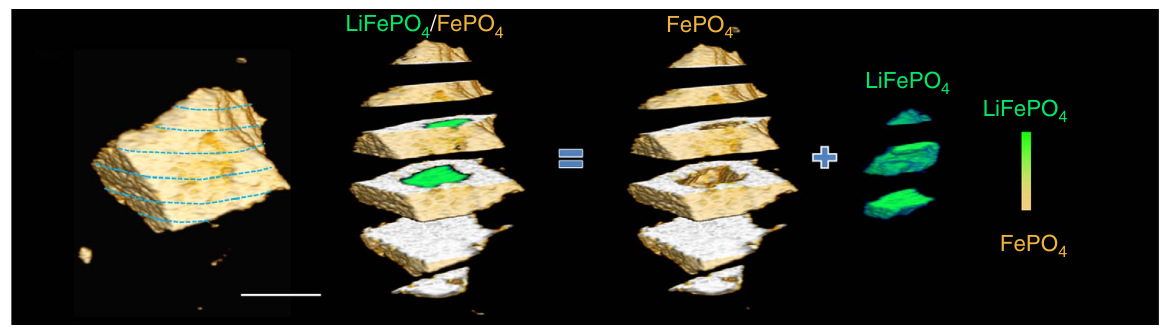
\includegraphics[width=\textwidth]{wang2016.png}
  \caption{Sliced view of \ce{LiFePO4} at highly delithiated
    state. The sliced view reveals 3D internal core-shell phase
    distribution. Scale bar, \SI{10}{\micro\metre}. Reprinted from
    reference\cite{wang2016}, licensed under
    \href{https://creativecommons.org/licenses/by/4.0/}{CC-BY 4.0}.}
  \label{figure:wang2016}
\end{figure}


\subsection{Structural Imaging}

% Intoroduction to structural imaging
\hl{RFC: Does this intro section read well with the ``methods'' description?}

Even though chemical oxidation state is of primary interest in
electrochemical reactions, it is not the only factor affecting
performance: structural changes can have a significant impact on the
kinetics of the underlying transformation. For example, site-mixing in
layered materials is known to impede lithium diffusion\cite{xu2016-2},
which reduces the power capability of the cathode. These and other
defects are not captured when measuring oxidation state, but are well
suited to investigation by diffraction-based techniques. As a result,
the applications presented here nicely complement the absorbance-based
chemical imaging presented above.

% Ex-situ diffraction mapping of LFP (that one figure that everyone cites)
Little work has been done on diffraction mapping of lithium-ion
cathodes. The most well-known example comes from Liu et
al.\cite{liu2010}, where the authors used synchrotron radiation to map
the surface of an electrode recovered from a partially charged
prismatic cell, shown in figure \ref{figure:liu2010}. However, this
work was carried out at coarse spatial resolutions (several
\si{\micro\meter}), compared to the nanoscale resolution of the other
microscopic mechanisms discussed in this Perspective. Nonetheless,
valuable information was gathered at the scale of the whole
electrode. Indeed, at high rates, they found a strong gradient in the
phase distribution along the direction of current flow from the
connector tab. The choice of a two-phase material (\ce{LiFePO4}) means
the phase distribution within a large electrode is unlikely to change
dramatically once the driving force is removed and the electrode is
removed from the cell, and therefore enabled the ex situ measurements
to produce meaningful data.

\begin{figure}
  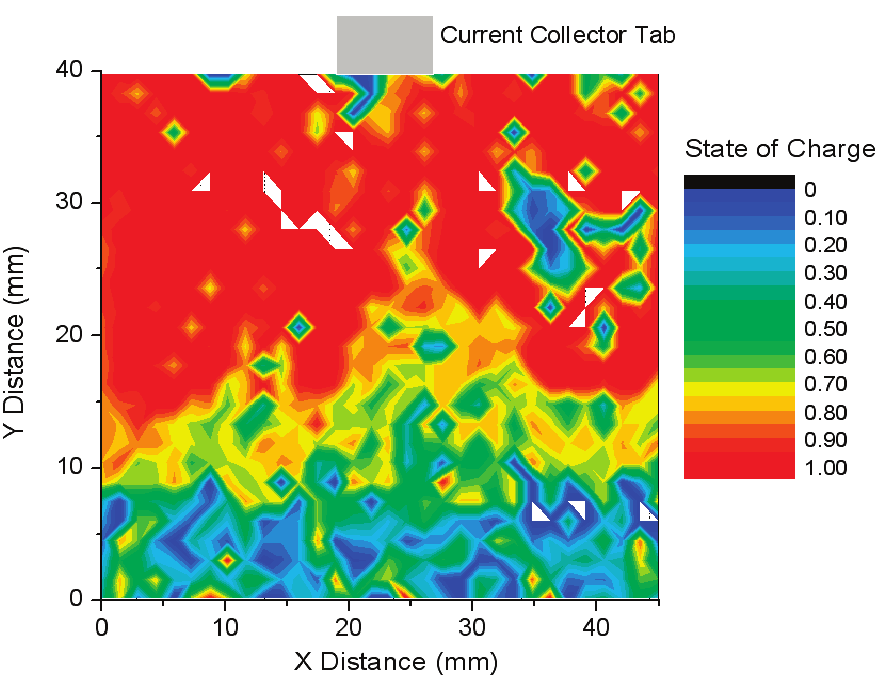
\includegraphics[width=\textwidth]{liu2010.png}
  \caption{\ce{FePO4} phase concentration profile of the prismatic
    electrode at 50\% state-of-charge.\cite{liu2010}}
  \label{figure:liu2010}
\end{figure}

% In-situ 3D LCO HE-XRD
Structural imaging is compatible with tomographic reconstruction.
%% A different approach does not limit the diffracted signal, but rather
%% uses a tomographic setup to acquire diffraction projections and
%% reconstruct the 3D volume.
Jensen et al.\ analyzed coin-cell and 18650-cell batteries using
tomography and high-energy diffraction\cite{jensen2015}. Line scans
were performed across the battery and at angles spanning \ang{180}
using a two-dimensional detector. The end result could
\emph{potentially} be a full two-dimensional diffraction pattern at
every position on the reconstructed slice (figure
\ref{figure:jensen2015}). In practice, the authors first integrated
each projection pattern azimuthally to a one-dimensional diffractogram
and then performed a reconstruction for each scattering vector length,
$q$. The two-dimensional diffraction pattern contains texture and
strain information that is lost when dimensionality is
reduced\cite{bobhe}. This feature was exploited by the authors by
separately integrating radially to map inhomogeneities in the
preferred orientation of the \ce{LiCoO_2} cathode material. The
\SI{70}{KeV} radiation used passes easily through the case material,
allowing the measurements to be performed in situ (though not
operando), avoiding any effects caused by disassembly of the cell.

\begin{figure}
  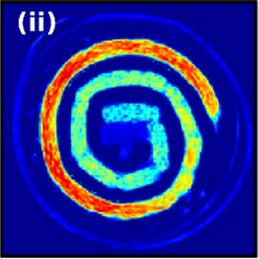
\includegraphics[width=\textwidth]{jensen2015.png}
  \caption{Data collected for cycled Ni-MH cell showing intensity at
    $q = \SI{1.36}{\per\angstrom}$, representing the cathode
    phase.\cite{jensen2015} Copyright The Authors 2015, Published by
    ECS. Creative Commons Attribution 4.0 License
    (\href{http://creativecommons.org/licenses/by/4.0/}{CC-BY}). Full
    text: \url{http://jes.ecsdl.org/content/162/7/A1310.full}}
  \label{figure:jensen2015}
\end{figure}

% 3D operando mapping of LFP using HE-XRD
The penetrating power of high energy X-rays can make for a very
compelling operando experiment since the cell does not have to be
modified, allowing conventional coin cells to be used. Strobridge et
al.\ mapped the volume of a \ce{LiFePO_4} cathode in this
way\cite{strobridge2015}. The incoming beam was scanned along the
width and/or height of the cell while a collimator between the sample
and detector allowed the authors to discriminate which gauge volume
along the beam was being probed (see figure
\ref{figure:strobridge2015}). The use of energy dispersive diffraction
meant that the collimator did not limit the range of scattering
vectors ($q$) being sampled. This feature allowed for direct mapping
of the entire volume. With this technique, a clear relationship
between electrode depth and state of charge was observed, leading to
valuable conclusions about the rate-limited steps in the reaction
mechanism. They also uncovered inhomogeneities across the width of the
electrode and used their measurements to validate a model exploring
the effects of electrode porosity.

\begin{figure}
  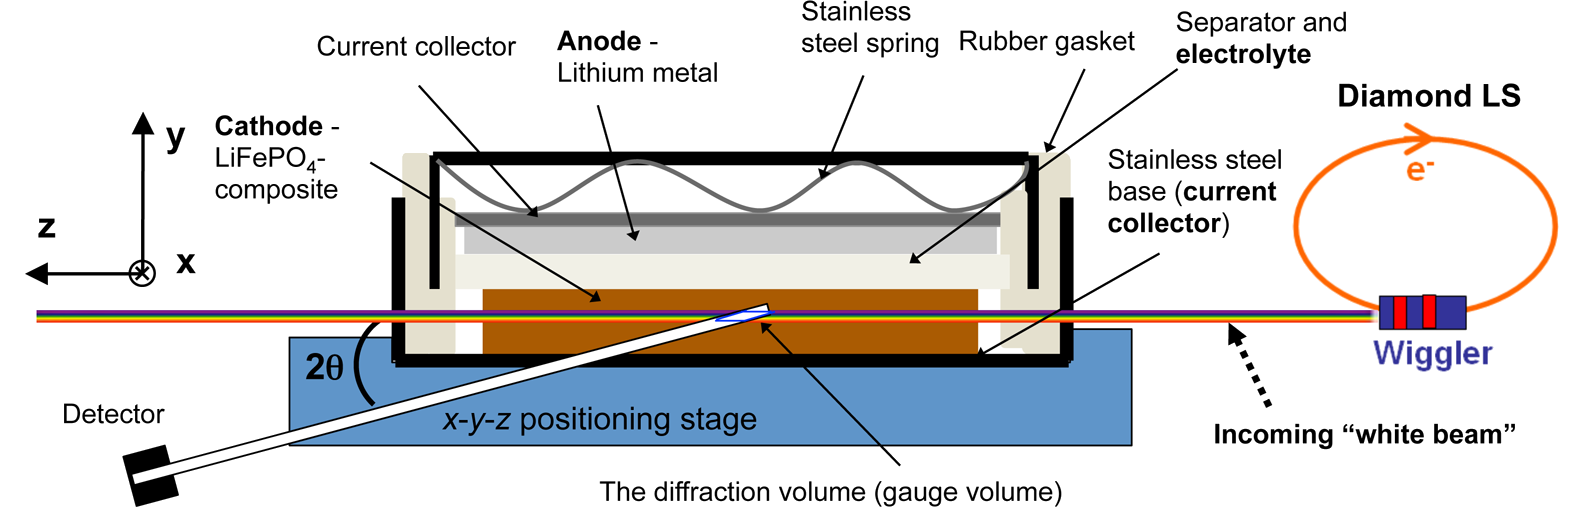
\includegraphics[width=\textwidth]{strobridge2015.png}
  \caption{\latin{In situ} EDXRD setup at the Diamond Light Source and the
    cross section of a coin-cell battery placed on an x-y-z position
    stage. X-rays penetrate the stainless steel casing and the
    diffracted X-rays are detected at a fixed angle.\cite{strobridge2015}}
  \label{figure:strobridge2015}
\end{figure}

Using a microprobe of \SI{1.7}{\micro\meter}, Zhang et al.\ probed
individual nanoscale \ce{LiFePO4} crystallites in operando. Slight
rotation of the sample illuminated several crystallites that satisfied
the diffraction condition. Each crystallite was separately resolved
because it was represented by a unique spot on the diffraction ring in
the two-dimensional diffraction pattern. By following each of those
spots through (dis)charge, the homogeneity and nature of the phase
transformation was examined. They found that at a slower rate of
(dis)charge the phase transformation occurs more homogeneously and
gradually, while faster rates see the advent of defined phase
boundaries\cite{zhang2015-2}.

% CDI (Ulvestad papers)
A similar strategy, relying on resolving crystallites through unique
diffraction spots in the Debye ring, was also applied to
\emph{coherent} Bragg diffraction, this time using
\ce{LiNi_{0.5}Mn_{1.5}O_4} as the case study\cite{singer2014}. The
power of this contrast mode, however, is exemplified by studies where
phenomena within a particle are resolved through reconstructions of
the three-dimensional volume, known as \emph{coherent diffraction
  imaging} (CDI). The specifics of the technique are also well suited
to mapping strain within the particle. Ulvestad et al.\ released a
series of papers using this technique. They first demonstrated its
validity by mapping the strain and displacement of material within a
particle\cite{ulvestad2014}. The strain evolution of
\ce{LiNi_{0.5}Mn_{1.5}O_4} was studied during charge/discharge and it
was shown that significant gradients exist right before the phase
transformation, shown in figure
\ref{figure:ulvestad2014-2}\cite{ulvestad2014-2}. In a separate
experiment, they used strain maps to infer the existence of
crystallographic defects within the crystallite and observed that
these defects move as a function of
charge-state\cite{ulvestad2015}. They were able to characterize the
dislocation by studying the displacement field around
it. Additionally, they quantified strain anisotropy, leading to the
proposal of a hinge-like structure between the unit-cell layers that
moves more freely once sufficient lithium is removed. Based on similar
observations made during discharge, it was shown that an initial
lithium-rich phase expands throughout the particle, rather than
multiple nucleation sites appearing; this result suggests that within
a single particle, the reaction pathway was close to thermodynamic
equilibrium in the conditions employed.

\begin{figure}
  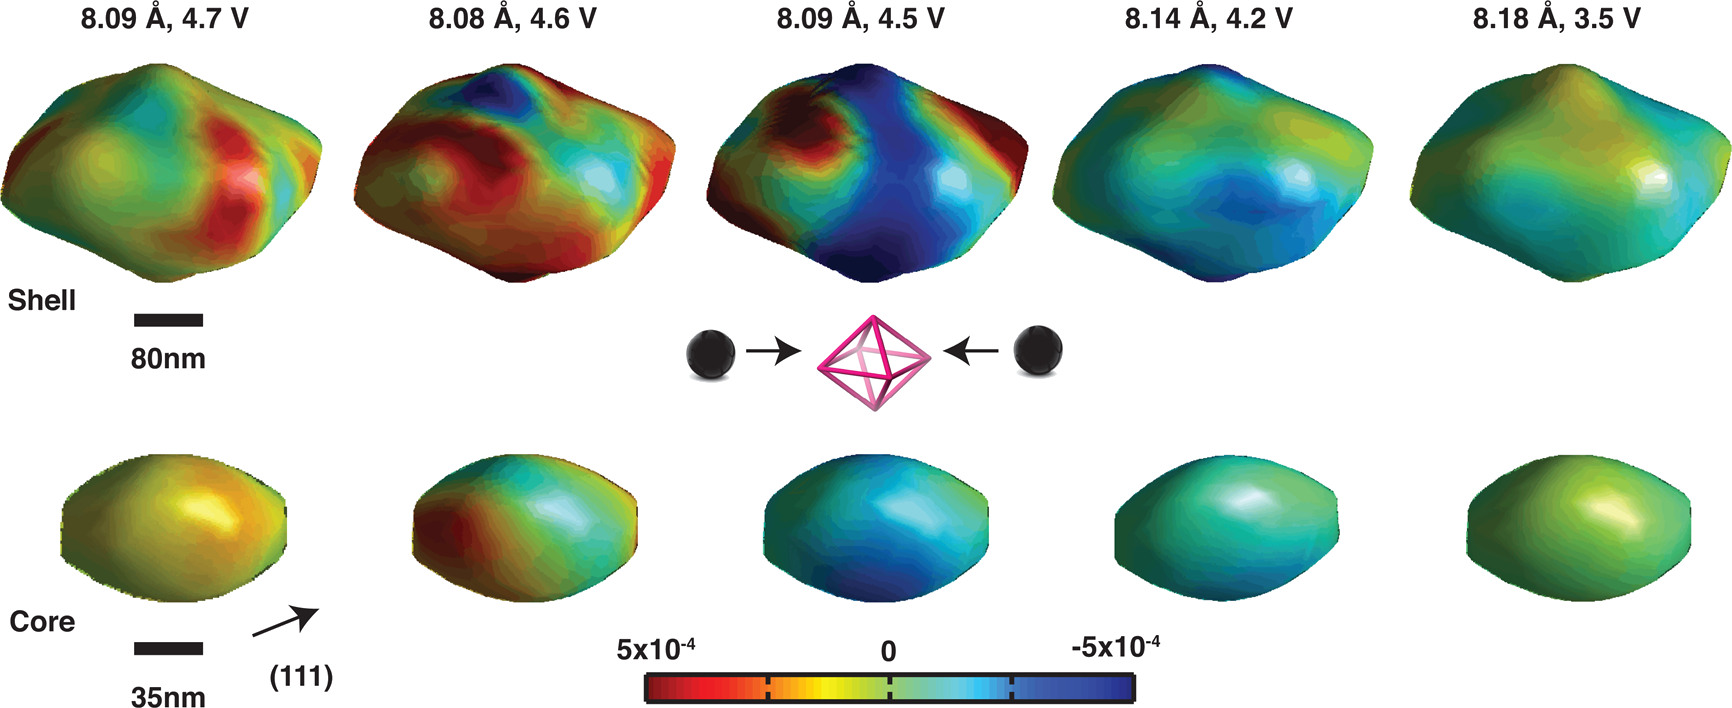
\includegraphics[width=\textwidth]{ulvestad2014-2}
  \caption{Isosurface projections of strain evolution in
    \ce{LiNi_{0.5}Mn_{1.5}O4} nanoparticle. The shell and core both
    show inhomogeneous strain during discharge. Images are labeled by
    their respective lattice constant values and open circuit
    voltages. The highest lattice strain occurs immediately prior to
    the phase transformation.\cite{ulvestad2014-2}}
  \label{figure:ulvestad2014-2}
\end{figure}


\section{Future Outlook}

The impact that X-ray imaging and mapping have already had in our
understanding of electrochemical reactions relevant to batteries is
significant. This perspective demonstrates that it is currently
possible to resolve chemical phenomena at the level of individual
particles, at resolutions as low as \SI{10}{nm}, and, in some case,
while the material is subject to working conditions. However, the
wealth of techniques presented here and the incipience of these
approaches lead to the conclusion that researchers are only beginning
to exploit the information that can be collected. We have emphasized
the importance of appropriately defining the goals of the experiment
in terms of chemical, spatial and temporal resolution. The three
cannot currently be attained at the same time in an experiment that is
directly relevant to function, with compromises leading to loss of
chemical information in most cases. It is also important to recognize
and understand the interaction between the beam and the material,
especially when molecules sensitive to radiation, such as the organic
solvents in a battery electrolyte, are present. This understanding is
currently extremely rudimentary, so systematic studies should be
incentivized.

When it comes to operando measurements, further improvements in
measurement protocols and cell design are necessary. Data analysis ``on
the fly'' would provide valuable input to the experimenter in terms of
defining the chances of success of the experiment and creating options
for data minimization and experiment optimization. When it comes to
experimental environments, the higher the resolution desired, the
heavier the need for engineering cells that notably differ from
conventional battery setups such as coin or even prismatic cells. This
design often imposes conditions that are not representative, or where
quantitative electroanalysis simultaneous to the observations is not
possible, inducing a critical loss of information. Further, given the
ultimate goal of guiding improvements in battery performance, it is
important that the design of operando cells takes into account the
need to preserve the fidelity of the electrochemical responses
to those that define function in a device.

As the community increases its awareness of the unique capabilities of
X-ray microscopes, it is expected that their use in battery research
will continue to grow. Since chemical imaging is only possible at a
synchrotron, this growth will contribute to a vibrant and diverse user
community. The fact that synchrotron scientists continue to improve
existing setups and design new modes of imaging will contribute to the
presence of X-ray chemical imaging and mapping in battery research. In
this context, the availability of access to the synchrotron facilities
where the measurements are performed is likely to become an even more
pronounced limiting factor to be tackled by the agencies managing the
facilities. A solution would involve improvements in the flux and
brightness of the X-ray source to decrease measurement times. Indeed,
many facilities are in the process of upgrading their storage rings to
provide X-rays to enable techniques with increased complexity, while
shortening the measurement times for those that are already possible
today. The National Synchrotron Light Source II (NSLS-II) has now
replaced the original NSLS at Brookhaven. Additionally, the Advanced
Photon Source (APS), Advanced Light Source, Stanford Synchrotron
Radiation Lightsource, and Cornell High Energy Synchrotron Source
(United States), as well Deutsches Elektronen-Synchrotron and European
Synchrotron Radiation Facility in Europe, and Spring-8 in Japan all
have plans for upgrading in the future, though many of these are still
in very early planning stages. These improvements promise brighter and
more coherent X-rays. The APS-U project also promises X-ray beams that
will be much smaller in the horizontal direction, allowing more of the
beam to be focused on the sample for imaging applications. The
coherence of the X-rays is critical for ptychography and CDI; having
pervasive access to coherent radiation will make these imaging
techniques faster and more efficient than today. Increased brightness
will shorten the time needed to acquire a data-set of sufficient
quality for analysis. These developments would bring experiments
without compromises in any of the dimensions of resolution closer to
reality. In other words, it would translate into an increase in the
time resolution of operando experiments without sacrificing spatial or
chemical resolution and will facilitate the next generation of
high-impact experiments. Both operando and three-dimensional analyses
have demonstrated their ability to generate insights that would
otherwise go unnoticed: combining them in a robust and practical way
will likely be at the forefront of battery imaging techniques. These
developments will surely drastically improve the way that we are able
to define relevant reactions, at the level of molecules to
architectures, providing vital inputs for the design of devices that
break current barriers of performance.

\section{Acknowledgement}
This work was supported as part of the NorthEast Center for Chemical
Energy Storage (NECCES), an Energy Frontier Research Center funded by
the U.S. Department of Energy, Office of Science, Basic Energy
Sciences under Award \# DE-SC0012583.

\bibliography{refs}

\bibstyle{achemso}

\section{Biographies}

\subsection{Mark Wolf}
Mark Wolf is a Ph.D.\ candidate at the University of Illinois Chicago
performing research on cathode materials using ptychography and
operando X-ray microscopy. He received a Bachelor of
Science from Western Michigan University in 2008 with a dual-major in
chemistry and music.

\subsection{Brian M.\ May}

Brian May is a Ph.D.\ candidate at the University of Illinois at
Chicago in Dr.\ Jordi Cabana's group. Prior to his time at UIC, he
received his B.S.\ in chemistry from Loyola University Chicago in
2013, and researched allosteric activation mechanisms and protein
crystal structures with Dr.\ Miguel Ballicora and Dr.\ Dali Liu. His
current research focuses on developing new synchrotron techniques for
applications in understanding the chemical reactions of battery
cathode materials.

\subsection{Jordi Cabana}

Jordi Cabana is an Assistant Professor at the Department of Chemistry
of the University of Illinois at Chicago. Prior to his appointment at
UIC, he was a Research Scientist at Lawrence Berkeley National
Laboratory (USA), from 2008 until 2013. Prof.\ Cabana completed his
Ph.D.\ in Materials Science at the Institut de Ci\`encia de Materials de
Barcelona (Spain) in 2004, and worked in the Department of Chemistry
at Stony Brook University (USA) as a postdoctoral associate. He is
generally interested in the physical and inorganic chemistry of
materials, with emphasis on their redox and transport properties, and
a focus on applications in electrochemical energy storage. Members of
his group are frequent users of synchrotron techniques such as
diffraction, spectroscopy and microscopy.

\end{document}
